 %%%   DO NOT EDIT THIS SECTION  %%%

\section{Instrument}
\label{sec:instrument} %3
PICO meets all of its science-derived instrument requirements (STM)
with a single instrument: an imaging polarimeter with 21 frequency
bands centered between 21 and 799\,GHz. The instrument is built around
an all-aluminum two-reflector Dragone-style telescope
(\S\,\ref{sec:telescope}) with an internal aperture stop between the
primary and secondary. The focal plane is populated by 12,996
transition edge sensor (TES) bolometers (\S\,\ref{sec:focal_plane})
read out using a time-domain multiplexing scheme
(\S\,\ref{sec:detector_readout}). The instrument employs a single
science observing mode: fixed rotation-rate imaging while scanning the sky.

A V-groove radiator assembly provides passive cooling
(\S\,\ref{sec:radiative_cooling}). The instrument is configured inside
the shadow of the V-grooves, thermally and optically shielded from the
Sun. The sun shadow cone depicted in Fig.~\ref{fig:InstrumentCAD} is
$29\degree$. The angle to the Sun during the survey, $\alpha = 26\degree$
(\S\,\ref{sec:survey_design} \comor{and Fig.~\ref{fig:MissionDesignFigure}}), is supplemented with a margin of
$3\degree$ to account for the radius of the sun ($0.25\degree$), pointing
control error, design margin, and alignment tolerances.

The V-groove assembly is attached to the bipod struts that support the
instrument structural ring. The ring supports the primary reflector
and telescope box \comor{'Telescope box' is not a good terminology; telescope refers to all reflectors. suggest to change to 'cold box'; will need to change the label in the Figure}. The telescope box contains the actively cooled
components (\S\,\ref{sec:cadr}, \S\,\ref{sec:4kcooler}), including
the secondary reflector, the focal plane, and sub-kelvin adiabatic
refrigerator structures. Just inside the box, a thermal liner serves
as a cold optical baffle and aperture stop.

During the survey, the instrument is spun at 1 rpm
(\S\,\ref{sec:survey_design}). Spacecraft control is simplified by
mounting the instrument on a spinning spacecraft module, while a
larger non-spinning module houses most spacecraft subsystems
(\S\,\ref{sec:spacecraft}). Instrument elements that act as heat
sources are accommodated on the spinning module of the
spacecraft. Instrument integration and test (I\&T) is described in
\S\,\ref{sec:iandt}.



\subsection{Telescope}
\label{sec:telescope} %3.1

PICO telescope design is driven by a combination of science
requirements and physical volume limits. The science requirements are:
a large diffraction-limited field of view (DLFOV) sufficient to
support $\sim10^4$ detectors, arcminute resolution at 800~GHz, \comor{low 
spurious}
polarization, \comor{ and} low sidelobe response. All requirements
are met with PICO's 1.4\,m aperture modified open-Dragone design
(Fig.~\ref{fig:OpticsDiagram}). There are no moving parts in the PICO optical system.
\comor{we should take figure 19 out. It is not useful for the decadal panel. Can give reference to the Young etal. paper.}

\comor{this entire paragraph is not necessary}
More than 30 years ago Dragone analyzed the performance of several
off-axis systems and found solutions with low cross-polarization at
the center of the field of view and with stigmatism, or astigmatism
and coma, canceled to first order \citep{Dragone1978,Dragone1983a,Dragone1983b}. A number of recent suborbital CMB instruments
have used off-axis systems, and several began design optimization with
systems based on designs by Dragone \citep{Fargant2000,Swetz2011,Padin2008}.

The PICO optical design was selected following a trade study examining
cross-Dragone, Gregorian Dragone, and open-Dragone designs
\citep{Young2018}. \comor{We chose the open-Dragone because both the cross- and open-Dragone systems can accommodate the focal plane size required, while the Gregorian can not~\citep{deBernardis2018}, and because the open-Dragone is more compact and does not require more massive baffles that the cross-Dragone would require to overcome its sidelobes.}
\comor{The initial open-Dragone design has been modified by adding an aperture stop and adding corrections to the primary and secondary reflectors to enlarge the diffraction limited field of view.  The
detailed geometric parameterization of the PICO optical design is
described in \cite{Young2018}. }

\comor{ The two reflectors (270 cm $\times$ 205 cm primary and 160 cm $\times$ 158 cm secondary) are all-aluminum to minimize complexity. The highest frequency (900\,GHz) sets the surface accuracy requirement of the reflectors to $\sim \lambda/14 =24$\,$\mu$m. The focal ratio is 1.42. The primary is maintained at ambient temperature. A cold stop, between the primary and secondary reflectors, and the secondary reflector are actively cooled.  The slightly concave focal surface, which has a radius of curvature of 4.55\,m, is telecentric to within $0.12\degree$ across the entire FOV. }
%This results in a defocus of 0.1\,mm at the edge of a flat 10\,cm detector wafer, adding an RMS wavefront error of less than 3\,$\mu$m, which is negligible relative to PICO's shortest wavelength.

\comor{Stray light analysis of the PICO open-Dragone design using GRASP
confirms that the focal plane is protected from direct view of the sky, and that spillover
past the primary is suppressed by 80\,dB relative to the main lobe for
both co-pol and cross-pol beams. }

%The Gregorian Dragone has less diffraction-limited focal plane area than the open-Dragone \citep{deBernardis2018}, and is unable to support enough detectors to provide the required sensitivity. The cross-Dragone design has significant sidelobes that can be mitigated by baffles, but at the expense of added mass and volume.

\begin{figure}
\begin{center}
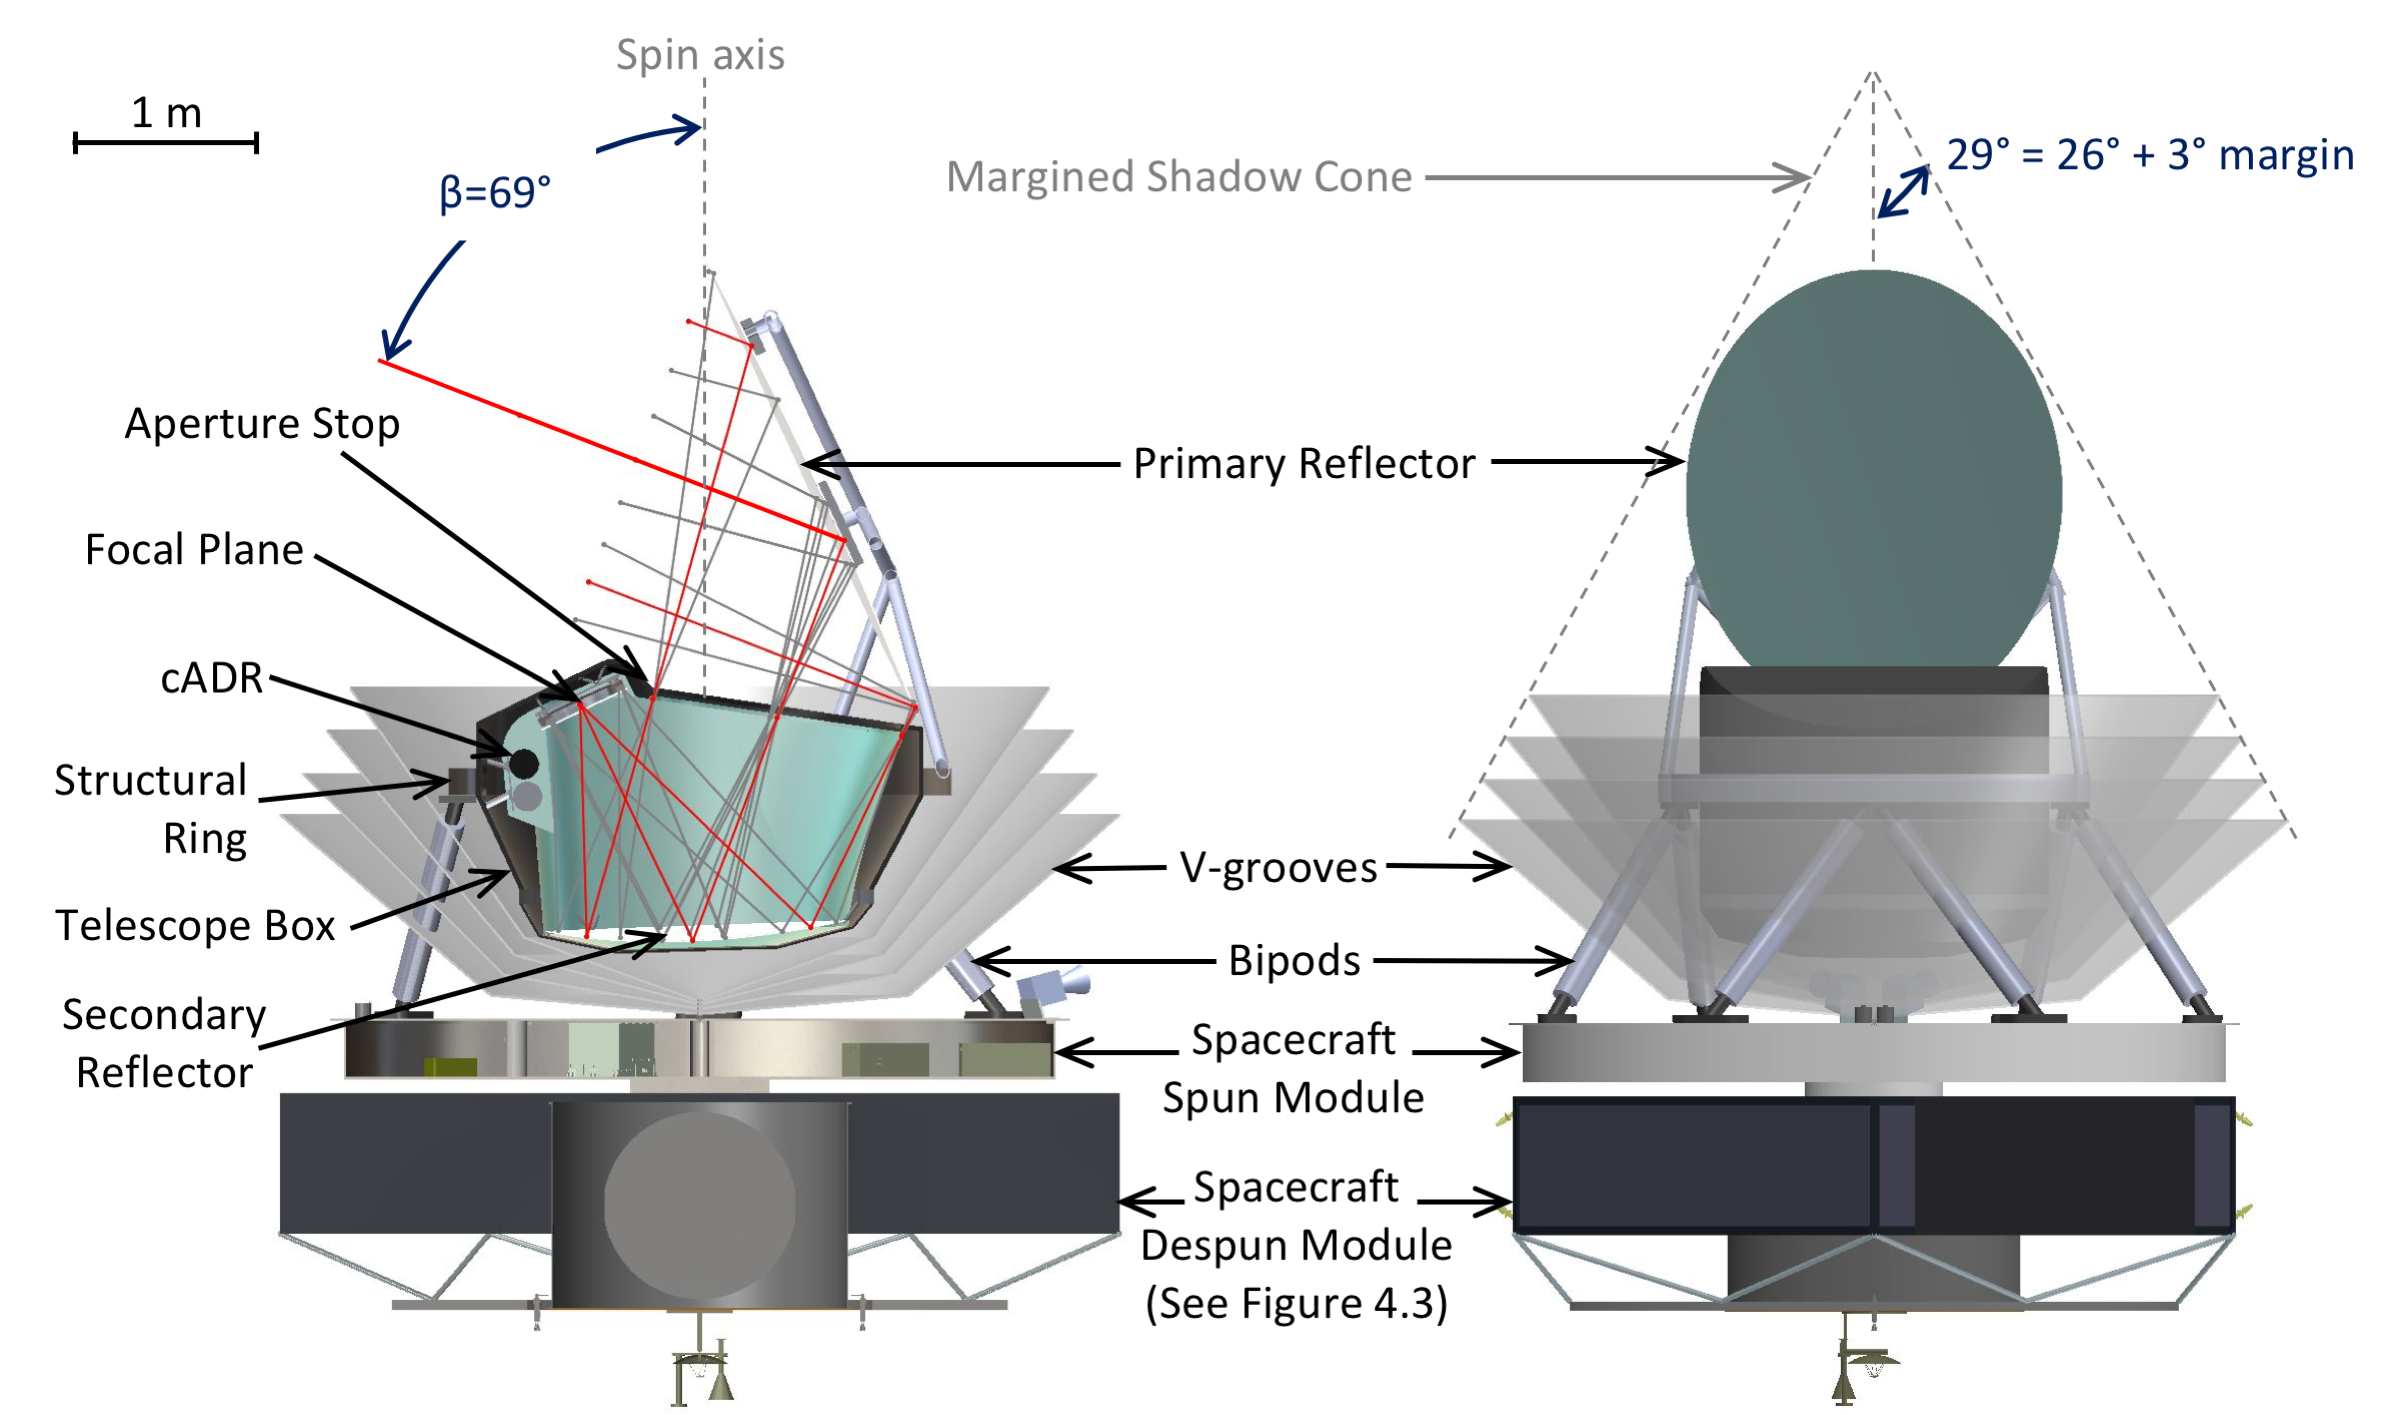
\includegraphics[width=6.25in]{figures/InstrumentCAD.png}
\caption{Detailed PICO instrument configuration. There are no moving or deployed parts. The spacecraft spun module accommodates warm instrument components: the 4\,K cooler compressor and drive electronics, the sub-K cooler drive electronics, and the detector warm readout electronics.\label{fig:InstrumentCAD}}
\end{center}
\end{figure}

\begin{figure}
\begin{center}
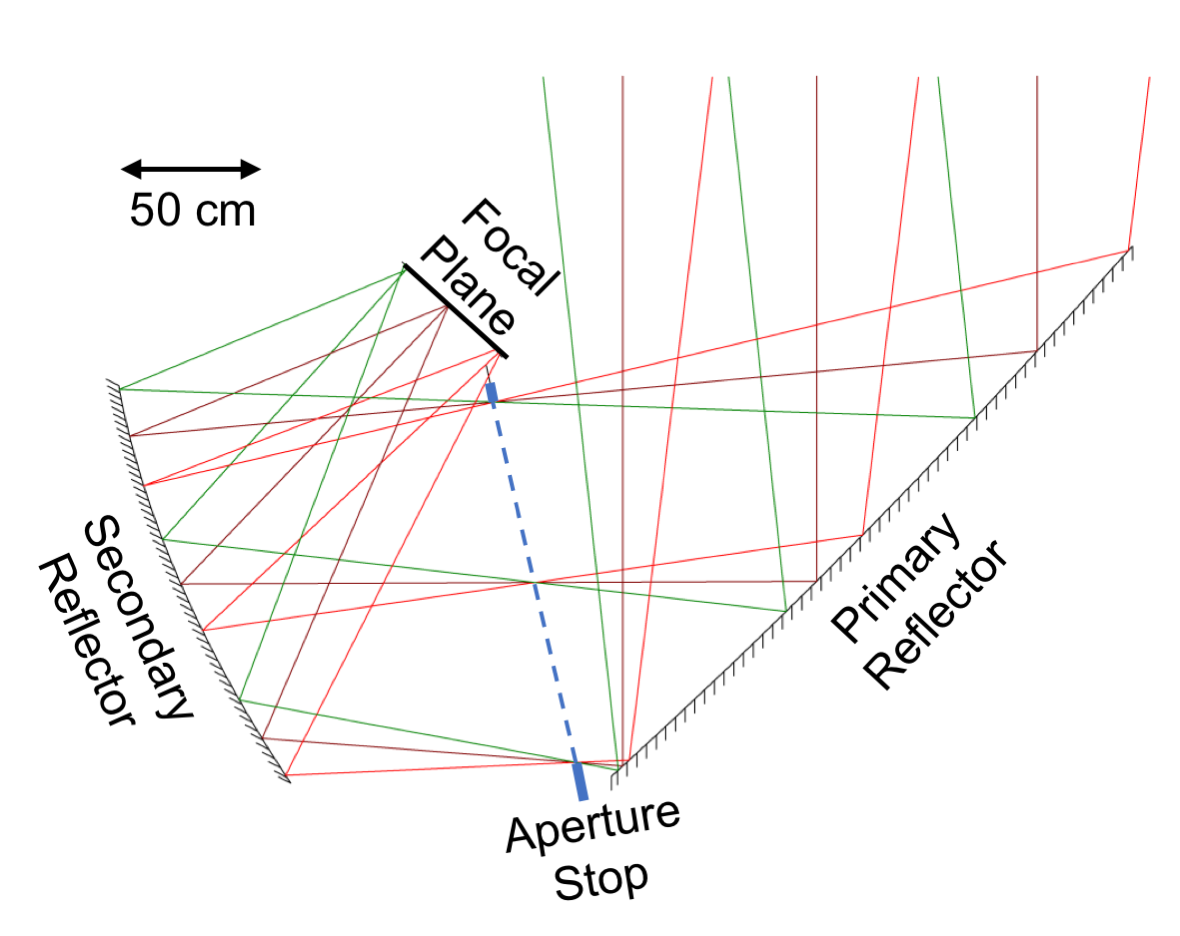
\includegraphics[width=3in]{figures/OpticsDiagram.png}
\caption{The optical system is compact.\label{fig:OpticsDiagram} \comor{this figure is not necessary}}
\end{center}
\end{figure}

\comor{replaced the entire red text below with the orange text above.}
\comred{
Stray light analysis of the PICO open-Dragone design using GRASP
confirms that the focal plane is protected from direct view of the sky 
(an advantage relative to the cross-Dragone system), that spillover
past the primary is suppressed by 80\,dB relative to the main lobe for
both co-pol and cross-pol beams. Relative to the cross-Dragone, an
open-Dragone also has a smaller f-number, so the volume constrained by
the shadow cone can accommodate a larger effective aperture. The
smaller f-number also reduces the physical focal plane size (for the
same number of pixels), reducing focal plane mass and consequently the
heat lift requirements on the active coolers (\S\,\ref{sec:thermal}).} 

\comred{
PICO's initial open-Dragone design follows Granet's method
\citep{Granet2001}, with f/1.42. An actively cooled circular aperture
stop is added between the primary and secondary reflectors to reduce
detector noise and shield the focal plane from stray
radiation. Distortions are then added to the primary and secondary
reflectors according to Dragone's published prescription
\citep{Dragone1983b} to eliminate coma and increase the DLFOV. The
detailed geometric parameterization of the PICO optical design is
described in \cite{Young2018}. }

\comred{replaced all the material below, with what's above
The PICO open-Dragone design follows Granet's method
\citep{Granet2001}, with f/1.42. An actively cooled circular aperture
stop is added between the primary and secondary reflectors to reduce
detector noise and shield the focal plane from stray
radiation. Distortions are then added to the primary and secondary
reflectors according to Dragone's published prescription
\citep{Dragone1983b} to eliminate coma and increase the DLFOV. The
detailed geometric parameterization of the PICO optical design is
described in \cite{Young2018}.}


\comred{
The two reflectors (270 cm $\times$ 205 cm primary and 160 cm $\times$ 158 cm secondary) are all-aluminum to minimize complexity. The highest frequency (900\,GHz) sets the surface accuracy requirement of the reflectors to $\sim \lambda/14 =24$\,$\mu$m. }

\comred{
The slightly concave focal surface, which has a radius of curvature of 4.55\,m, is telecentric to within $0.12\degree$ across the entire FOV. This results in a defocus of 0.1\,mm at the edge of a flat 10\,cm detector wafer, adding an RMS wavefront error of less than 3\,$\mu$m, which is negligible relative to PICO's shortest wavelength.}

\begin{figure}
\parbox{3in}{\centering
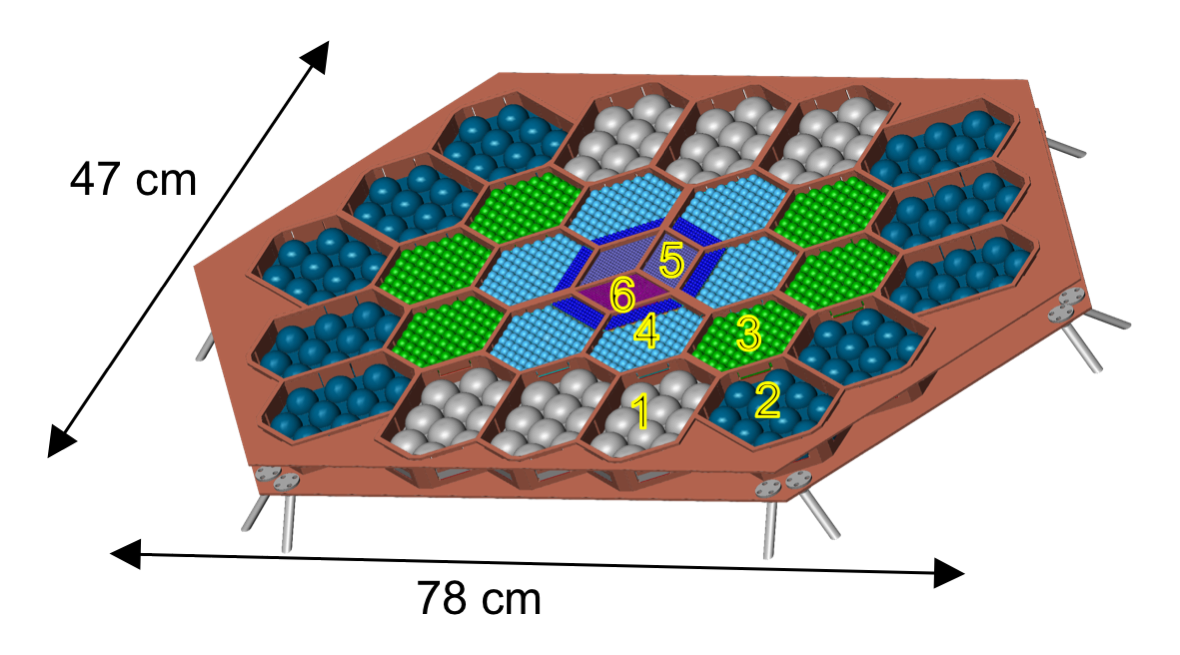
\includegraphics[width=3in]{figures/FocalPlaneMechanical.png}
}
\parbox{3.5in}{\centering
\caption{PICO focal plane. Detectors are fabricated on six types of tiles (shown numbered and colored to match first column in Table~\ref{tab:focal_plane}). The wafers are located on the focal plane such that higher frequency bands, which require better optical performance, are placed nearer to the center.\label{fig:FocalPlaneMechanical}}
}
\end{figure}

\begin{table}
\parbox{3.5in}{\centering
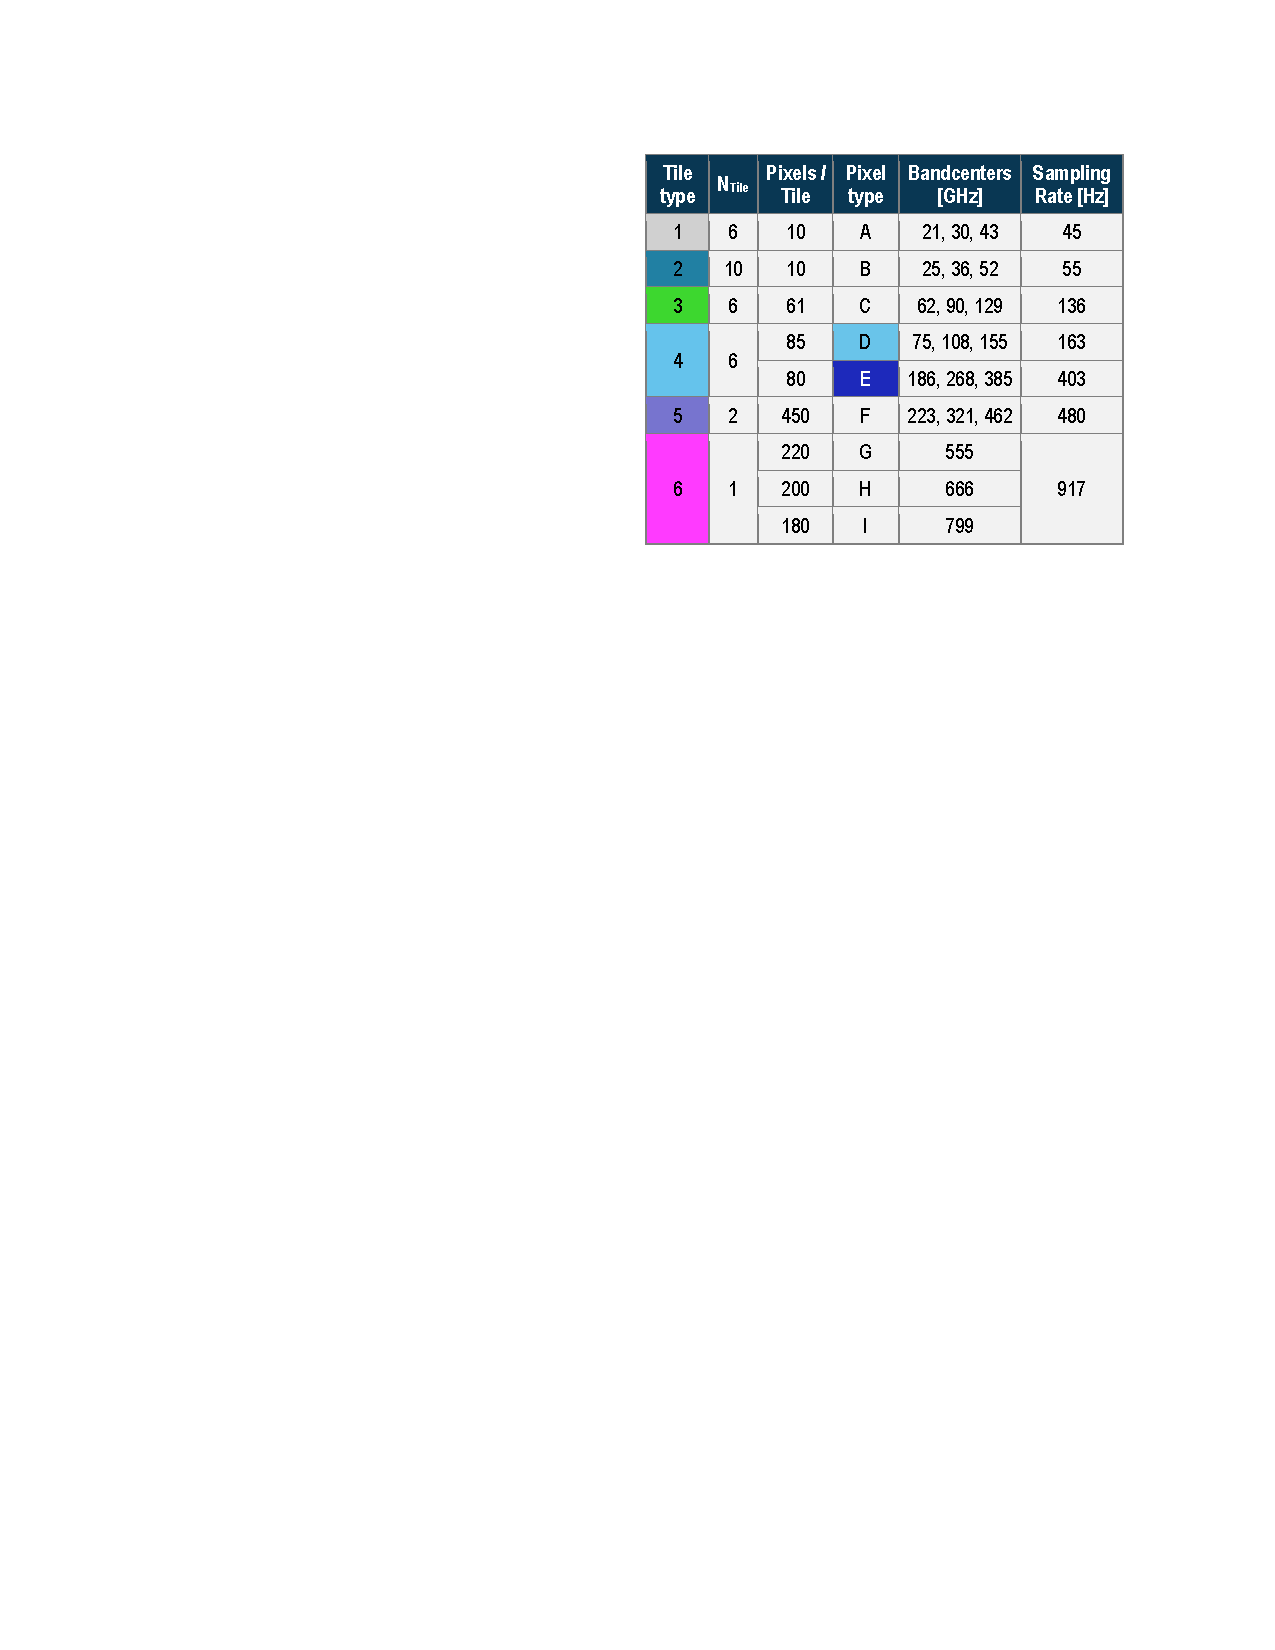
\includegraphics{tables/tab_focal_plane.pdf}}
\parbox{3in}{\centering
\caption{PICO makes efficient use of the focal area with multichroic pixels (three bands per pixel, \S\,\ref{sec:low_freq_det}). The sampling rate is based on the smallest beam (Table~\ref{tab:bands}), with 3 samples per FWHM at a scan speed $(360\degree/{\rm min})\sin(\beta=69\degree) = 336\degree/{\rm min}$. \label{tab:focal_plane}} }
\end{table}

\subsection{Focal plane}
\label{sec:focal_plane} %3.2

PICO's focal plane is populated by an imaging array of transition edge sensor (TES) bolometers observing in 21 overlapping 25\%-wide frequency bands with band centers ranging from 21 to 799\,GHz. Polarization is measured by differencing the signals from pairs of polarization-sensitive bolometers. A conceptual layout of the PICO focal plane is shown in Fig.~\ref{fig:FocalPlaneMechanical} and detailed in Table~\ref{tab:focal_plane}.
 
Modern mm/sub-mm detectors are photon-noise limited, so the primary approach to increase sensitivity is to increase the number of detectors. The PICO focal plane has 12,996 detectors, 175 times the number flown on the \planck\ mission, providing a breakthrough increase in sensitivity with a comparably sized telescope. This breakthrough is enabled by development and demonstration \comor{in} suborbital projects, which now commonly \comor{use} field arrays of $\sim10^4$ detectors. \comor{For example, SPT-3G is currently observing with ... and by the time PICO will enter phaseA the Simmons Observatory will have ... include citations.} 

%\comor{sinuous antenna-coupled multi-chroic pixels (SAMP). For each pixel, a lenslet made of alumina couples the radiation onto a broad-band polarization-sensitive sinuous antenna. On-wafer filters separate the broad-band radiation into three colors. Six transition edge sensor (TES) bolometers detect the three colors and 2 polarizations.}

\subsubsection{Low-frequency detectors}
\label{sec:low_freq_det} % 3.2.1

\comor{The majority of the PICO focal plane is populated with} multichroic pixels (MCPs)~\citep{Suzuki2014,Datta2014}, which make optimal use of the focal plane area by feeding \comor{several} photometric bands from a common broad-band antenna \comor{that is polarization sensitive. PICO has three bands, and thus there are} six bolometers per pixel.

Several competing optical coupling technologies have matured over the past ten years using horn-coupling~\citep{Duff2016}, antenna-array coupling \citep{BICEP2015}, and sinuous antenna/lenslet-coupling~\citep{Edwards2012}, delivering high optical efficiency over more than an octave of bandwidth \comor{I don't think this is correct. The antenna-array is not giving octave of bandwidth. It is not a multi-color option. not sure that the horn-coupling is giving an octave. Need to check}. Pixel size, number, and spacing is relatively agnostic to the coupling scheme, so multiple options are open to PICO (technology maturation plan described in
\S\,\ref{sec:detector_development}). \comor{I am not sure this is what we want to say.} For all of these schemes,
\comor{niobium microstrips mediate} the signals between the antenna and detectors, and
\comor{partition the wide} continuous bandwidth into narrow channels
using integrated micro-machined filter circuits~\citep{OBrient2013}.

\subsubsection{High-frequency detectors}
\label{sec:high_freq_det} % 3.2.2

PICO's highest three frequency channels are beyond the Niobium superconducting band-gap, rendering microstrip filters a poor solution for defining the optical passband. In this regime, PICO instead
measures a single band with each pixel using feedhorn-coupled
polarization-sensitive bolometers. Radiation is coupled through horns
directly to \comor{an absorber. TES bolometers detect the incident power.} 
The waveguide cut-off defines the lower edge of the band,
and quasi-optical metal-mesh filters define the upper edge. Numerous
experiments have successfully used similar approaches
\citep{Shirokoff2011,Bleem2012,Turner2001}. The technology maturation
required for PICO is described in \S\,\ref{sec:detector_development}.
\comor{is there any tech maturation? we need to point to Planck and Herschel here.}

\begin{table}[!pt]
\parbox{4.45in}{
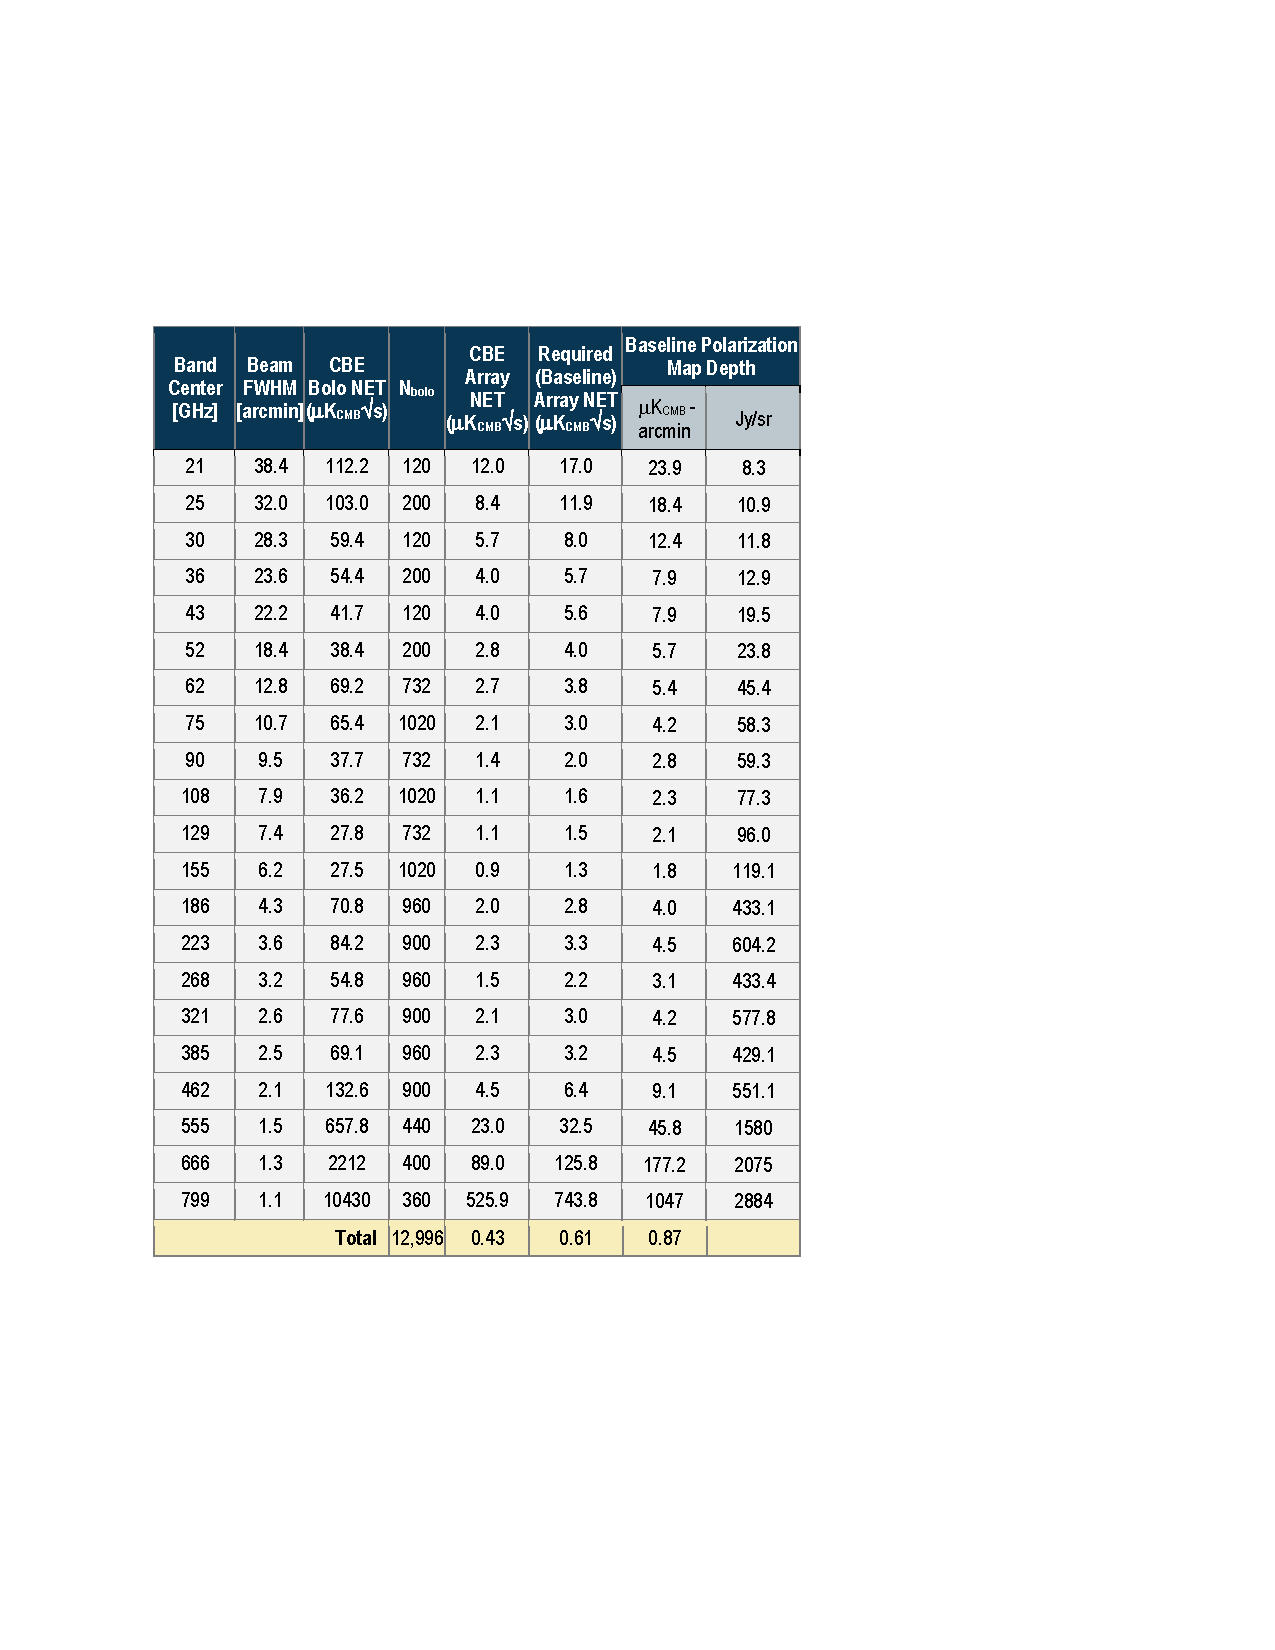
\includegraphics{tables/tab_bands.pdf} }
\parbox{2in}{
\caption{PICO measures in 21 broad overlapping frequency bands with band centers ($\nu_{\rm c}$) from 21\,GHz to 799\,GHz and bandwidth $\Delta\nu/\nu_{\rm c} = 25\,\%$. The beams are single mode, with FWHM sizes of $6.2' \times (155\,{\rm GHz}/\nu_{\rm c})$. The Current Best Estimate (CBE) per-bolometer sensitivity is background limited (\S\,\ref{sec:sensitivity}). The total number of bolometers for each band is equal to (number of tiles) $\times$ (pixels per tile) $\times$ (2 polarizations per pixel), from Table~\ref{tab:focal_plane}. Array sensitivity assumes $90\,\%$ detector operability, and meets the requirements of the baseline mission with $>40\,\%$ margin. The map depth assumes 5\,yr of full sky survey at $95\,\%$ survey efficiency, except the 25 and 30\,GHz frequency bands, which are conservatively excluded during 4\,hr/day Ka-band (26\,GHz) telecom periods (\S\,\ref{sec:ground_segment}).\label{tab:bands} } }
\end{table}

\subsubsection{Sensitivity}
\label{sec:sensitivity} %3.2.3

We developed an end to end noise model of the PICO instrument to
predict full mission sensitivity (Table~\ref{tab:bands}) and provide a
metric by which to evaluate mission design trades. The model considers
four noise sources per bolometer: photon, phonon, TES Johnson, and
readout (from both cold and warm readout electronics). To validate our
calculations, we compared two independent software packages that have
been \comor{validated through use on several current} CMB instruments. The calculations agreed within
1\% for both individual noise terms and for overall mission noise.

Laboratory experiments have demonstrated that TES detectors can be
made background limited in the low loading environment they would
experience at L2 \comor{is that true? reference? need to be careful. not sure that's been done for our loading levels. may need to cite Planck and spider} For PICO, the primary contributor to noise is the
optical load. The sources of optical load are the CMB, \comor{reflectors}, aperture stop, and low pass filters. The CMB and stop account for the majority of the optical load at all frequencies.
The CMB gives more than half the load in the middle and upper bands of
the multichroic pixels, but the stop dominates the load in the lowest
band of each pixel.  \comor{A detailed} description of the PICO noise model is available in
\citep{Young2018}\comor{; small differences with Table~\ref{tab:bands} are due} to refinements of the
component temperatures.  The sensitivity model assumes white noise at
all frequencies. \comor{removed the additional sentences; calibration uncertainties and systematics are *never* part of a sensitivity model. If we want to make this comment, which is a valid comment, it should be made elsewhere.} 
%, and does not include calibration uncertainties or estimates of other possible systematic effects, which are discussed in \S\,\ref{sec:2.7}. 

Sub-orbital submillimeter experiments have demonstrated TES detectors
that are stable to at least as low as 20\,mHz \citep{Rahlin2014},
meeting PICO's requirements for the proposed scan strategy
(\S\,\ref{sec:survey_design}).

\subsection{Detector readout}
\label{sec:detector_readout} %3.3

Suborbital experiment teams over the past ten years have chosen to use
voltage biased TESs because their current readout scheme lends itself
to SQUID-based multiplexing. Multiplexing reduces the number of wires
to the cryogenic stages and thus the total thermal load that the
cryocoolers must dissipate. This approach also simplifies the
instrument design.  In the multiplexing circuitry, SQUIDs function as
low-noise amplifiers and cryogenic switches. The current baseline for
PICO is to use a time-domain multiplexer (TDM), which assigns each
detector's address in a square matrix of simultaneously read columns,
and sequentially cycles through each row of the array
\citep{Henderson2016}. The PICO baseline architecture uses a matrix of
128 rows and 102 columns, requiring some technology maturation
(\S\,\ref{sec:readout_development}). The thermal loading on
the cold stages from the wire harnesses is subdominant to conductive
loading through the mechanical support structures.  Redundant warm
electronics boxes perform detector readout and instrument housekeeping
using commercially available ASICs. The readout electronics compress
the data before delivering it to the spacecraft. PICO detectors
produce a total of 6.1\,Tbits/day assuming 16\,bits/sample, sampling
rates from Table~\ref{tab:focal_plane}, and bolometer counts from
Table~\ref{tab:bands}. Suborbital work has demonstrated 6.2$\times$
compression of similar data \citep{EBEX2017}. \textit{Planck} HFI
typically achieved 4.7$\times$ compression in flight
\citep{Pajot2018,PlanckHFI2011}. PICO conservatively assumes
4$\times$.

\subsection{Thermal}
\label{sec:thermal} %3.4

\comor{The PICO focal plane is maintained at 0.1~K (\S\,\ref{sec:cadr})}, a temperature that simplifies TES bolometer design given the low optical loads expected. The \planck -HFI focal plane was also maintained at 0.1~K. To minimize
detector \sored{shot} noise due to instrument thermal radiation, the aperture
stop and reflectors are cooled using both active and radiative cooling
(\S\,\ref{sec:4kcooler}, \S\,\ref{sec:radiative_cooling}).  All
thermal requirements are met with robust margins
(Table~\ref{tab:cooler}).

\begin{table}
\parbox{4.0in}{
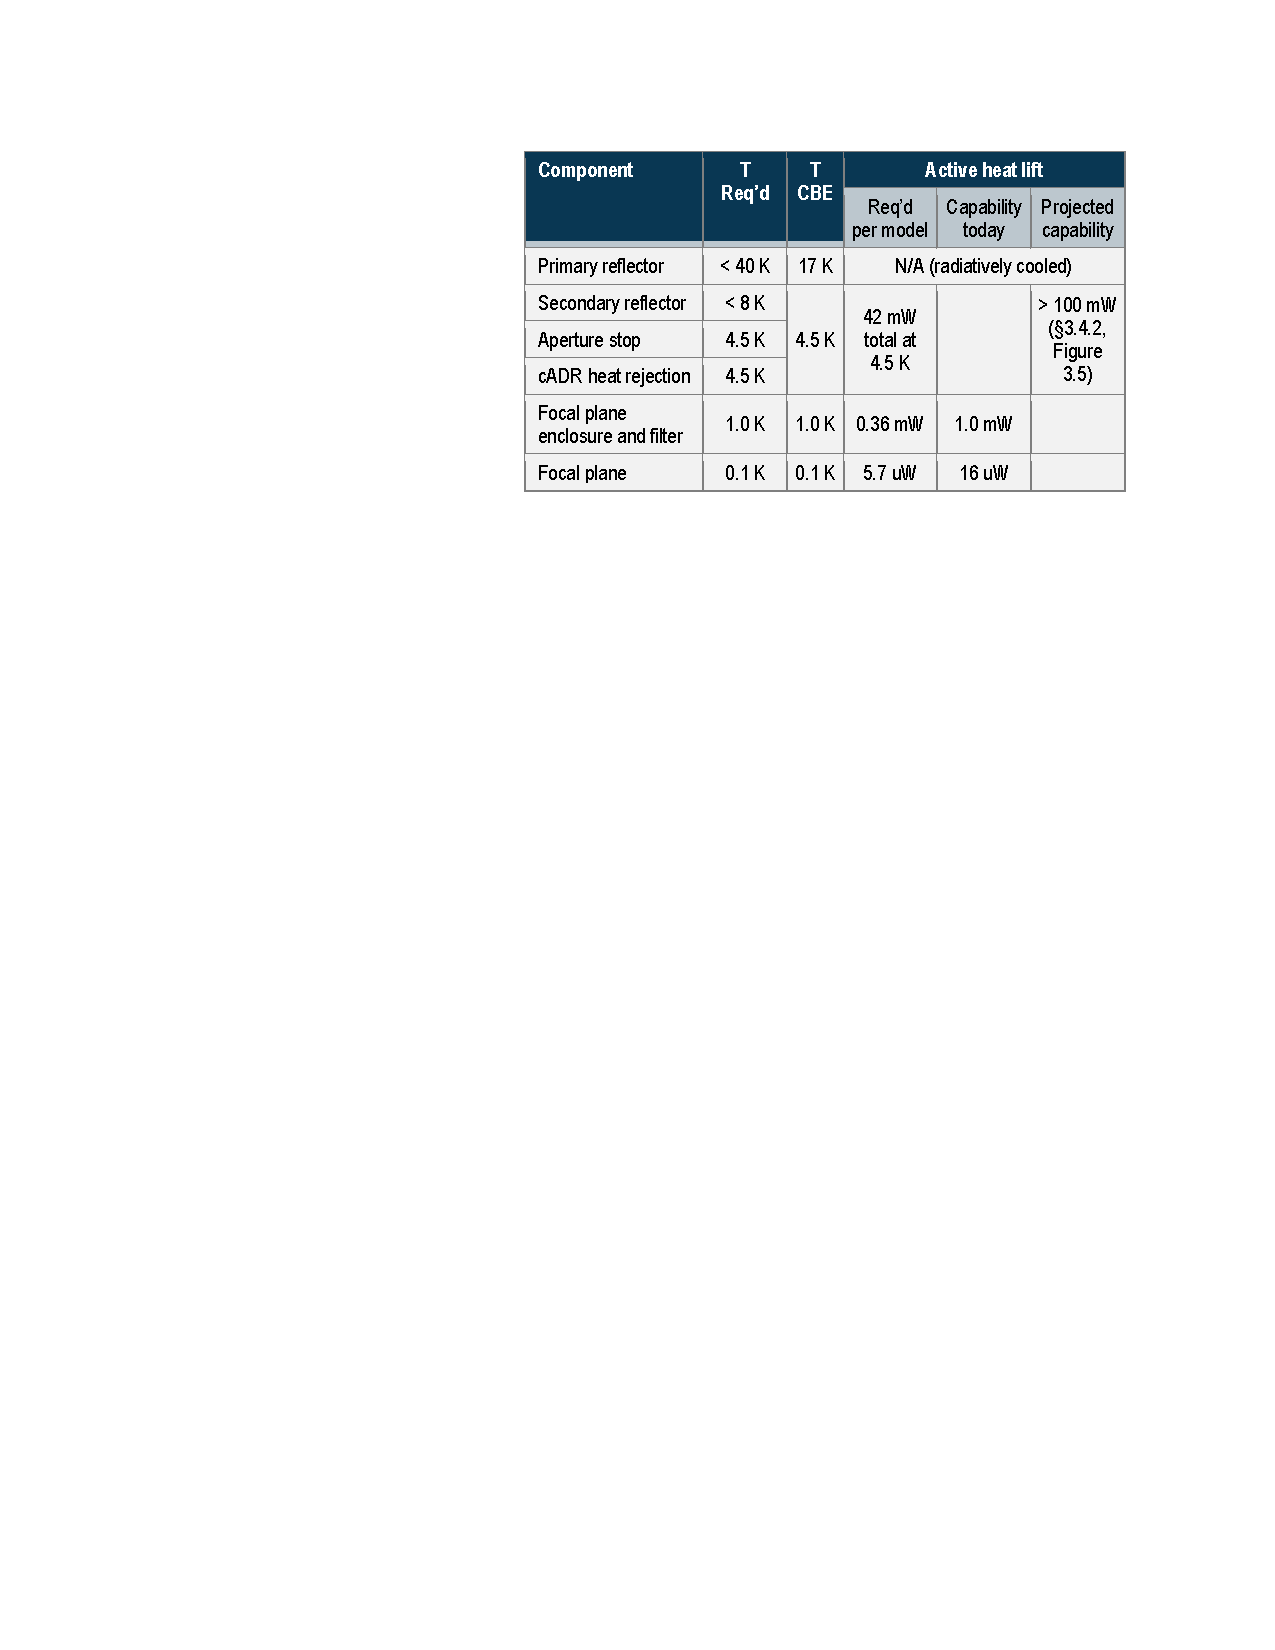
\includegraphics{tables/tab_cooler.pdf} }
\hspace{0.01in}
\parbox{2.5in}{
\caption{Projected cooler heat lift capabilities offer $>100\,\%$ margin, complying with community best practices \citep{Donabedian2003}. The cADR lift capability at 1\,K and 0.1\,K is from a Goddard quote. Both NGAS and Ball project $>100$\,mW lift capability at $4.5\,$K using higher compression-ratio compressors currently in development (\S\,\ref{sec:4kcooler}). The required loads were calculated using Thermal Desktop. Reference \citep{Ross2004} was used to estimate the thermal conductive loads through mechanical supports. In addition to the listed components, the total 4.5\,K heat load includes the intercept on the focal plane mechanical supports.\label{tab:cooler}} }
\end{table}

\begin{figure}[ht]
\parbox{4.0in}{
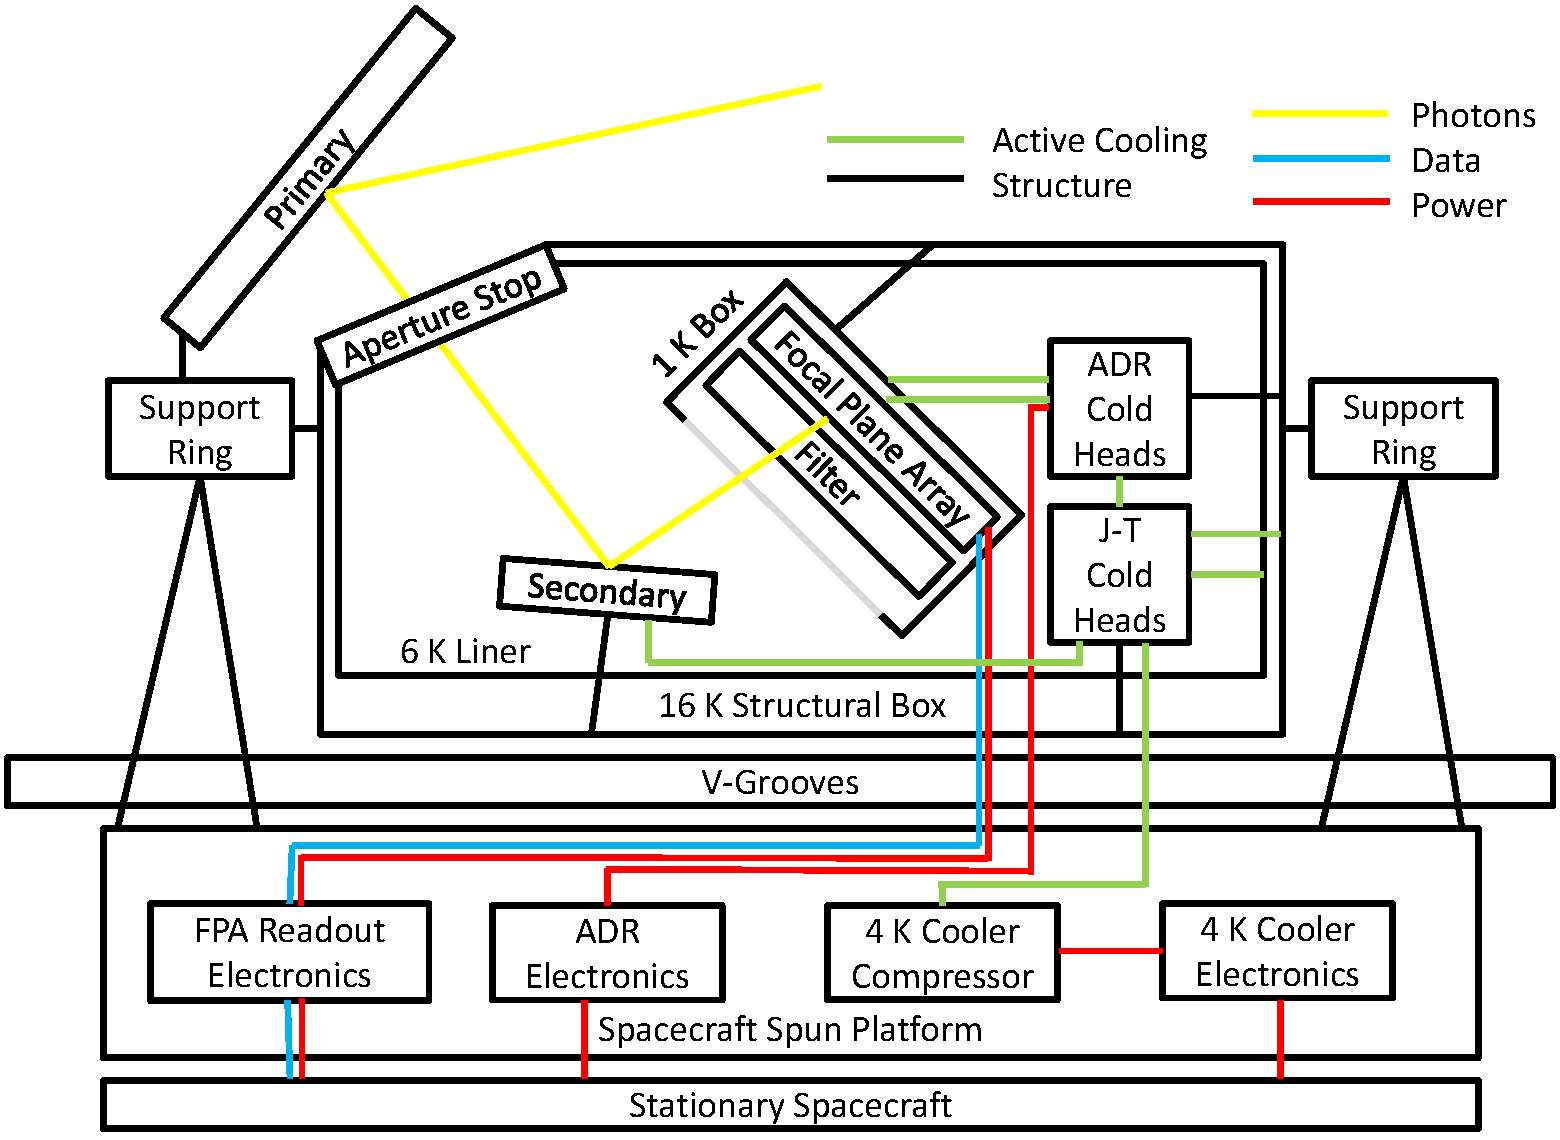
\includegraphics[width=4.in]{figures/ArchitectureBlockDiagram.pdf} }
\hspace{0.05in}
\parbox{2.45in}{
\caption{PICO instrument block diagram. Active coolers provide cooling
  to the focal plane, its box, the secondary reflector, and the
  thermal liner that acts as a cold aperture stop. Data from the focal
  plane flows to (redundant, cross-strapped) warm readout electronics
  on the spun module of the spacecraft
  bus.\label{fig:ArchitectureBlockDiagram}} }
\end{figure}


\subsubsection{cADR Sub-K Cooling}
\label{sec:cadr} %3.4.1

A multi-stage continuous Adiabatic Demagnetization Refrigerator (cADR)
cools the PICO focal plane to 0.1\,K and the surrounding enclosure,
filter, and readout components to 1\,K. The cADR employs three
refrigerant assemblies operating sequentially to absorb heat from the
focal plane at 0.1\,K and reject it to 1\,K. Additionally, the cADR
employs two assemblies operating sequentially to absorb this rejected
heat at 1\,K, cool other components to 1\,K, and reject heat at
4.5\,K. This configuration provides continuous cooling with small
temperature variations at both the 0.1\,K and 1\,K. Heat straps
connect the two cADR cold sinks to multiple points on the focal plane
assembly, which has high thermal conductance paths built in, to
provide spatial temperature uniformity and stability during
operation. Heat loads in the range of 20\,$\mu$W at 0.1\,K and 1\,mW
at 1\,K (time-average) are within the capabilities of current cADRs
developed by GSFC \citep{Shirron2012,Shirron2016}. The PICO sub-K
loads are estimated at less than half of this capability.

\subsubsection{4 K Cooler}
\label{sec:4kcooler} %3.4.2

A cryocooler system similar to that used on JWST to cool the MIRI
detectors \citep{Durand2008,Rabb2013} removes the heat rejected from
the cADR and cools the aperture stop and secondary reflector to
4.5\,K. Both NGAS (which provided the MIRI coolers) and Ball Aerospace
have developed such coolers under the NASA-sponsored Advanced
Cryocooler Technology Development Program \citep{Glaister2006}. NGAS
and Ball use slightly different but functionally-equivalent hardware
approaches. A 3-stage precooler (acoustic Stirling by NGAS or
mechanical Stirling by Ball) provides $\sim16$\,K precooling to a
separate circulated-gas loop driven by a similar compressor modified
for DC flow. The circulated-gas loop utilizes Joule--Thomson (J-T)
expansion, further cooling the gas to 4.5\,K. The entire precooler
assembly and the J-T circulator compressor are located on the warm
spacecraft, with relatively short tubing lengths conducting the gas
flow from the precooling point to the J-T expansion point. All waste
heat rejected by the cooler compressors and drive electronics is
transferred to the spacecraft heat rejection system. Unlike JWST, the
PICO cooler does not require deployment of the remote cold head.

The J-T expansion point is located close to the cADR heat rejection
point, thereby providing the lowest temperature to the
cADR. Subsequent to cooling the cADR, the gas flow intercepts
conducted heat to the focal plane enclosure, then cools the aperture
stop and the secondary reflector before returning in counterflow to
the circulation compressor.  Model-based projections indicate that the
coolers delivered for MIRI could meet the PICO 4.5\,K heat lift
requirement with $>100\,\%$ margin with minimal changes: the replacement
of the $^4$He gas used for MIRI with $^3$He, plus resizing of the gas
counterflow heat exchangers to take advantage of the $^3$He

\begin{figure}
\parbox{3.5in}{\centering
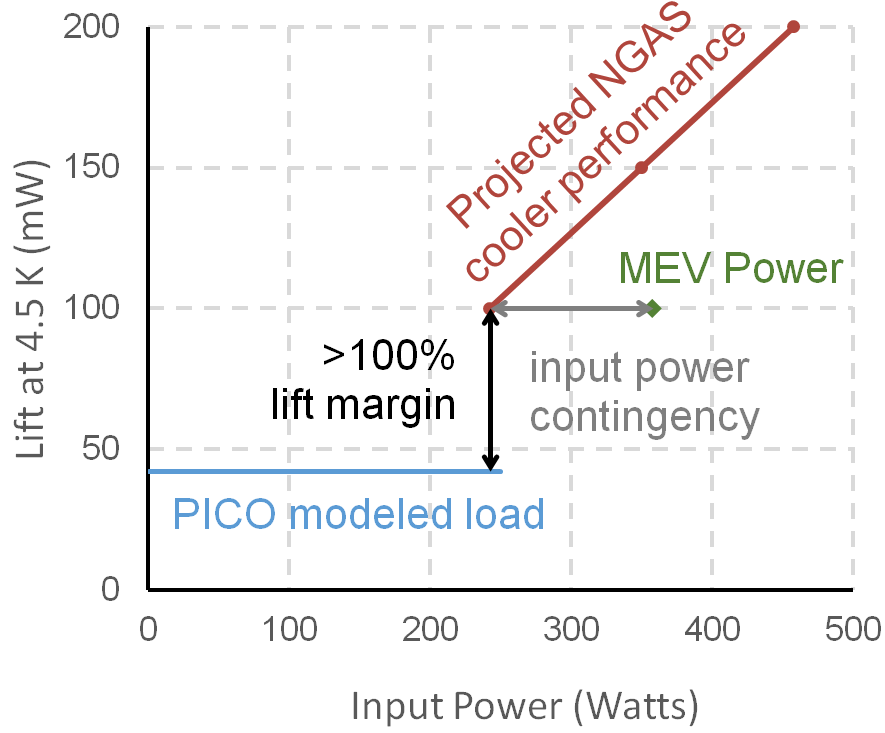
\includegraphics[width=3in]{figures/CoolerFigure.png}}
\parbox{3.0in}{
\caption{Projected performance of the NGAS cooler using a multi-stage
  compressor and $^4$He \citep{Rabb2013} meets PICO's requirements
  with $>100\,\%$ margin. PICO conservatively carries additional input
  power contingency on the efficiency of the
  cooler.\label{fig:CoolerFigure}} }
\end{figure}

It is highly likely that a better solution will be available before
Phase~A. NGAS and Ball are actively working on increasing the flow
rate and compression ratio of the J-T compressor, which should result
in significantly higher system efficiency, and in greater heat-lift
margin above the PICO requirement. These improvements entail the
implementation of well-known techniques (standard thermal
engineering). The NGAS multi-stage J-T compressor has completed
PDR-level development, and is expected to reach CDR level well before
needed for PICO. Projected performance is shown in Fig.~\ref{fig:CoolerFigure}. The
Ball approach started with a larger compressor, required less
modification to achieve comparable performance, and eliminated the
cold bypass-precooling valve that was problematic for MIRI. The Ball
approach uses $^3$He, while the NGAS approach uses $^4$He. Both employ
re-optimized gas heat exchangers (trivial engineering changes).


\subsubsection{Radiative cooling}
\label{sec:radiative_cooling} %3.4.3

A set of four V-groove radiators provides passive cooling. The
outermost of the four V-groove shields shadows the interior shields
from the Sun. The V-grooves radiate to space, each reaching
successively cooler temperatures. The V-groove assembly is
mechanically supported from the spacecraft bus by attachment to the
low-conductance bipod struts that also carry the mechanical loads of
the structural ring (Fig.~\ref{fig:InstrumentCAD}). The V-groove
assembly provides a cold radiative environment to the primary
reflector, structural ring, and telescope box, so radiative loads on
those elements are smaller than the conductive loads through the
mechanical support structures.


\subsection{Instrument integration and test}
\label{sec:iandt} % 3.5

PICO Instrument I\&T planning benefits greatly from heritage
experience with the \textit{Planck} HFI instrument \citep{ Pajot2010}.

PICO will screen detector wafer performance prior to selection of
flight wafers and focal plane integration. The cADR and 4\,K
cryocooler will be qualified prior to delivery. The relative alignment
of the two reflectors under thermal contraction will be
photogrammetrically verified in a thermal vacuum (TVAC) chamber.

PICO will integrate the flight focal plane assembly and flight cADR in
a dedicated sub-kelvin cryogenic testbed. Noise, responsivity, and FPU
temperature stability will be characterized using a representative
optical load for each frequency band (temperature-controlled
blackbody). Polarimetric and spectroscopic calibration will be
performed.

The focal plane will be integrated with the reflectors and structures,
and alignment verified photogrammetrically at cold temperatures in a
TVAC chamber.  The completely integrated observatory will be tested in
TVAC to measure parasitic optical loading from the instrument, noise,
microphonics and radio-frequency interference (RFI).

\section{Design reference mission}
\label{sec:design_reference} %4

\subsection{Concept of operations}
\label{sec:operations} %4.1

The PICO concept of operations is similar to that of the successful
\textit{WMAP} \citep{Bennett2003} and \textit{Planck} \citep{Tauber2010} missions. After launch,
PICO cruises to a halo orbit around the Earth--Sun L2 Lagrange point
(\S\,\ref{sec:mission_design}). En route, a 2-week decontamination period is followed by
instrument cooldown. After in-orbit checkout is complete, PICO begins
the science survey.

PICO has a single science observing mode, surveying the sky
continuously for 5 years using a pre-planned repetitive survey pattern
(\S\,\ref{sec:survey_design}). Instrument data are compressed and stored on-board, then
returned to Earth in daily 4-hr Ka-band science downlink passes
(concurrent with science observations). Because PICO is observing
relatively static Galactic, extragalactic, and cosmological targets,
there are no requirements for time-critical observations or data
latency. Presently, there are no plans for targets of opportunity or
guest observer programs during the prime mission. The PICO instrument
does not require cryogenic consumables (as the \textit{Planck} mission did),
permitting consideration of mission extension beyond the prime
mission.

\begin{figure}[!b]
  \begin{minipage}[b]{0.65\textwidth}
    \begin{center}
    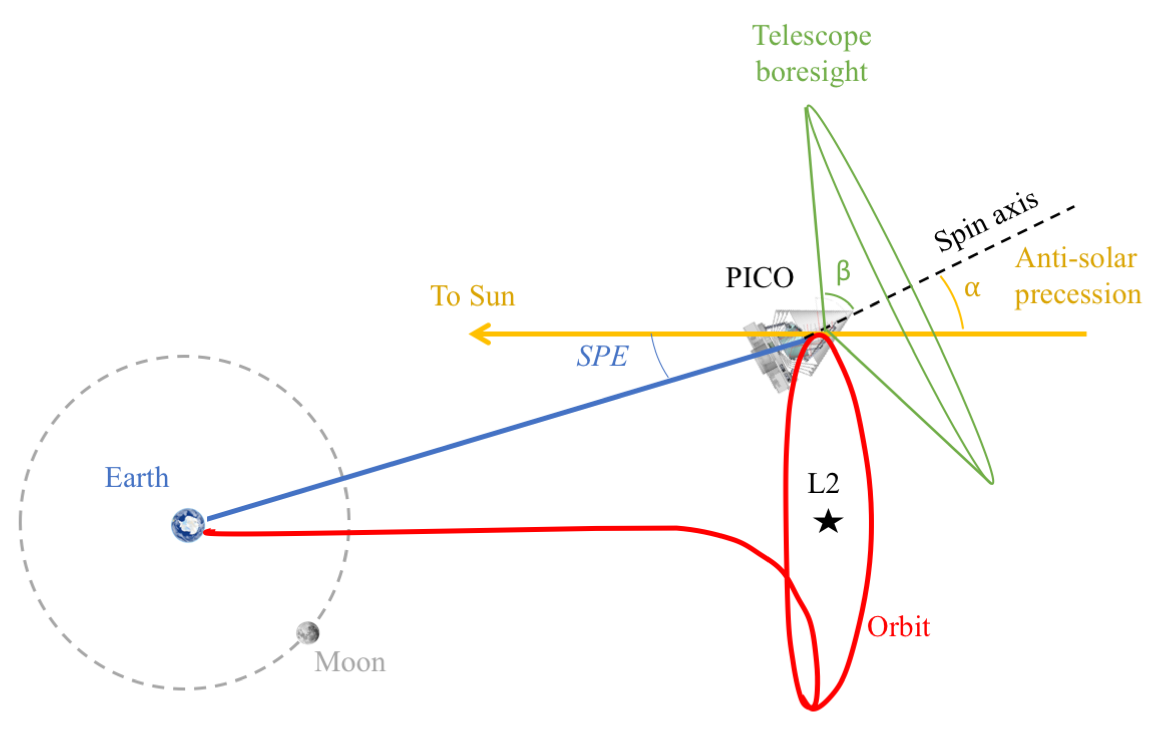
\includegraphics[width=4in]{figures/MissionDesignFigure.png}
\caption{PICO surveys by continuously spinning the instrument about a
  precessing axis.\label{fig:MissionDesignFigure}}
   \end{center}
  \end{minipage}
  \hspace{0.15in}
  %
  \begin{minipage}[b]{0.29\textwidth}
    \begin{center}
    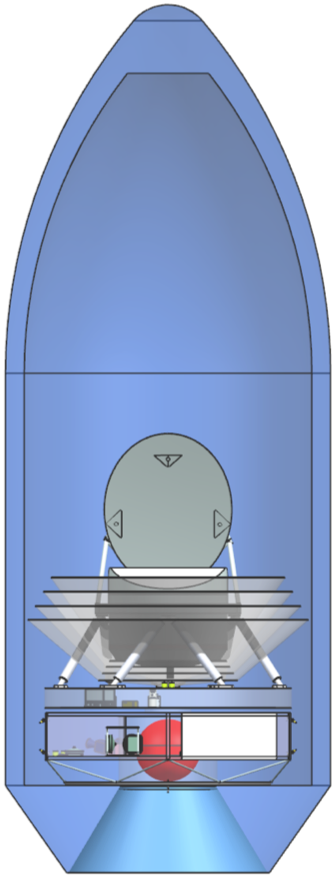
\includegraphics[width=0.7in]{figures/InFairing.png}
\caption{PICO is compatible with the Falcon~9.\label{fig:InFairing}}
    \end{center}
  \end{minipage}
\end{figure}

% \begin{figure}
% \begin{center}
% 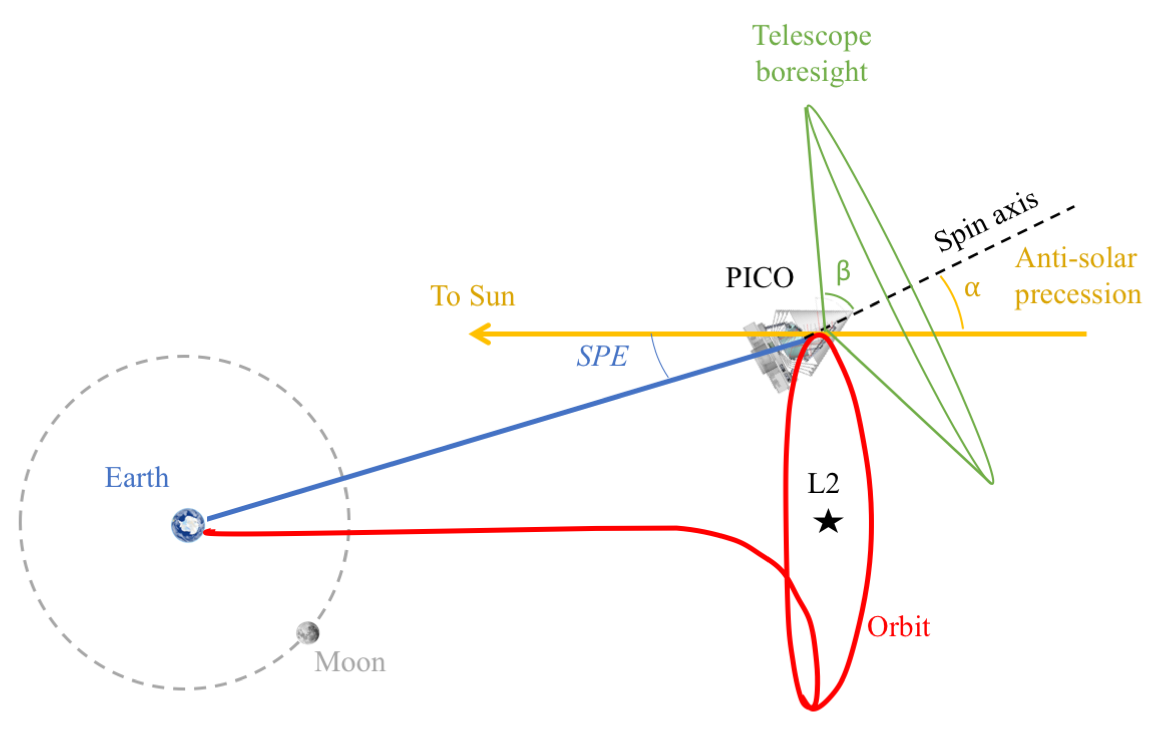
\includegraphics[width=3in]{figures/MissionDesignFigure.png}
% \caption{PICO surveys by continuously spinning the instrument about a
%   precessing axis.\label{fig:MissionDesignFigure}}
% \end{center}
% \end{figure}


% \begin{figure}
% \begin{center}
% 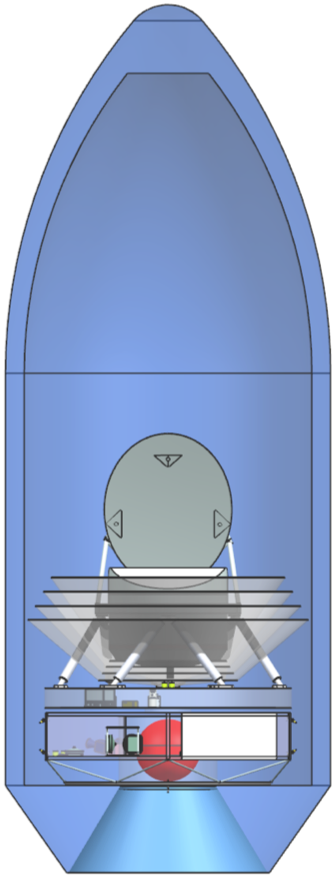
\includegraphics[width=1in]{figures/InFairing.png}
% \caption{PICO is compatible with the Falcon~9.\label{fig:InFairing}}
% \end{center}
% \end{figure}

\subsubsection{Mission design and launch}
\label{sec:mission_design} %4.1.1

PICO performs its science survey from a halo orbit around the
Earth--Sun L2 Lagrange point. Predecessor missions \textit{Planck} and
\textit{WMAP} both operated in L2 orbits.

L2 orbits provide favorable survey geometry (relative to Earth orbits)
by mitigating viewing restrictions imposed by terrestrial and lunar
stray light. The PICO orbit around L2 is small enough to ensure than
the Sun--Probe--Earth (SPE) angle is less than $15\degree$. This
maintains the telescope boresight $>70\degree$ away from the Earth
(Fig.~\ref{fig:MissionDesignFigure},
$70\degree = 180\degree -\alpha - \beta - \rm{SPE}$).  High data rate
downlink to the Deep Space Network (DSN) is available from L2 using
near-Earth Ka bands. L2 provides a stable thermal environment,
simplifying thermal control. The PICO orbit exhibits no post-launch
eclipses.
 
NASA requires that Probes be compatible with an Evolved Expendable
Launch Vehicle (EELV). For the purpose of this study, the Falcon~9
\citep{SpaceX2015} is used as the reference
vehicle. Fig.~\ref{fig:InFairing} shows PICO configured for launch in a
Falcon~9 fairing. PICO's launch mass is well within the Falcon~9
capability.

Insertion to the halo manifold and associated trajectory correction
maneuvers (TCMs) require 150\,m\,s$^{-1}$ of total $\Delta v$ by the
spacecraft. The orbital period is $\sim6$\,months. Orbit maintenance
requires minimal propellant (statistical
$\Delta v\sim 2$\,m\,s$^{-1}$\,year$^{-1}$). There are no disposal
requirements for L2 orbits, but spacecraft are customarily
decommissioned to heliocentric orbit.


\subsubsection{Survey design}
\label{sec:survey_design} %4.1.2
 
PICO utilizes a highly repetitive scan strategy to map the full
sky. During the survey, PICO spins with a period
$T_{\rm spin} = 1$\,min about a spin axis oriented $\alpha=26\degree$
from the anti-solar direction (Fig.~\ref{fig:MissionDesignFigure}). This spin axis
is forced to precess about the anti-solar direction with a period
$T_{\rm prec}= 10$\,hr. The telescope boresight is oriented at an
angle $\beta=69\degree$ away from the spin axis. This $\beta$ angle is
chosen such that $\alpha + \beta > 90\degree$, enabling mapping of all
ecliptic latitudes. The precession axis tracks with the Earth in its
yearly orbit around the Sun, so this scan strategy maps the full sky
(all ecliptic longitudes) within 6 months.

PICO's $\alpha=26\degree$ is chosen to be substantially larger than
the \textit{Planck} mission's $\alpha$ angle ($7.5\degree$) to
mitigate systematic effects by scanning across each sky pixel with a
greater diversity of orientations \citep{Hu2003}. Increasing $\alpha$
further would decrease the sun-shadowed volume available for the
optics and consequently reduce the telescope aperture size. A
deployable sun shade was considered, but not baselined.

The instrument spin rate, selected through a trade study, matches that
of the Planck mission. The study balanced low-frequency ($1/f$) noise
subtraction (improves with spin rate) against implementation cost and
heritage, pointing reconstruction ability (anti-correlated with spin
rate), and data volume (linearly correlated with spin rate). The $\ell=2$
quadrupole power spectral mode appears in the data timestream at $2\ell
\sin(\beta)/T_{\rm spin} = 60$\,mHz \citep{Wallis2017}. Detector noise is stable down to
these frequencies (\S\,\ref{sec:sensitivity}). A destriping mapmaker applied in data
post-processing effectively operates as a high-pass filter, as
demonstrated by \textit{Planck} \citep{Kurki-Suonio2009}. PICO's spin axis
precession frequency is $>400\times$ faster than that of \textit{Planck}, greatly
reducing the effects of any residual $1/f$ noise by spreading the
effects more isotropically across pixels.

\subsection{Ground segment}
\label{sec:ground_segment} %4.2

The PICO Mission Operations System (MOS) and Ground Data System (GDS)
can be built with extensive reuse of standard tools. The PICO concept
of operations is described in \S\,\ref{sec:survey_design}. There are
no time critical events, and no driving data latency
requirements. Routine orbit maintenance activities are required
roughly every three months (\S\,\ref{sec:mission_design}). The payload
consists of a single instrument with a single science observing mode
(a repetitive survey pattern, \S\,\ref{sec:survey_design}).
 
All space-ground communications, ranging, and tracking are performed
by the Deep Space Network (DSN) 34\,m Beam Wave Guide (BWG). X-band is
used to transmit spacecraft commanding, return engineering data, and
provide navigation information. Ka-band is used for high rate return
of science data (150\,Mb/s transfer; 130\,Mb/s information rate after
CCSDS encoding). The instrument produces 6.1\,Tb/day, which is
compressed to 1.5\,Tb/day (\S\,\ref{sec:detector_readout}). Daily
4\,hr DSN passes return PICO data in 3.1\,hr, with the remaining
0.9\,hr available as needed for retransmission or missed-pass
recovery.


\begin{figure}
\begin{center}
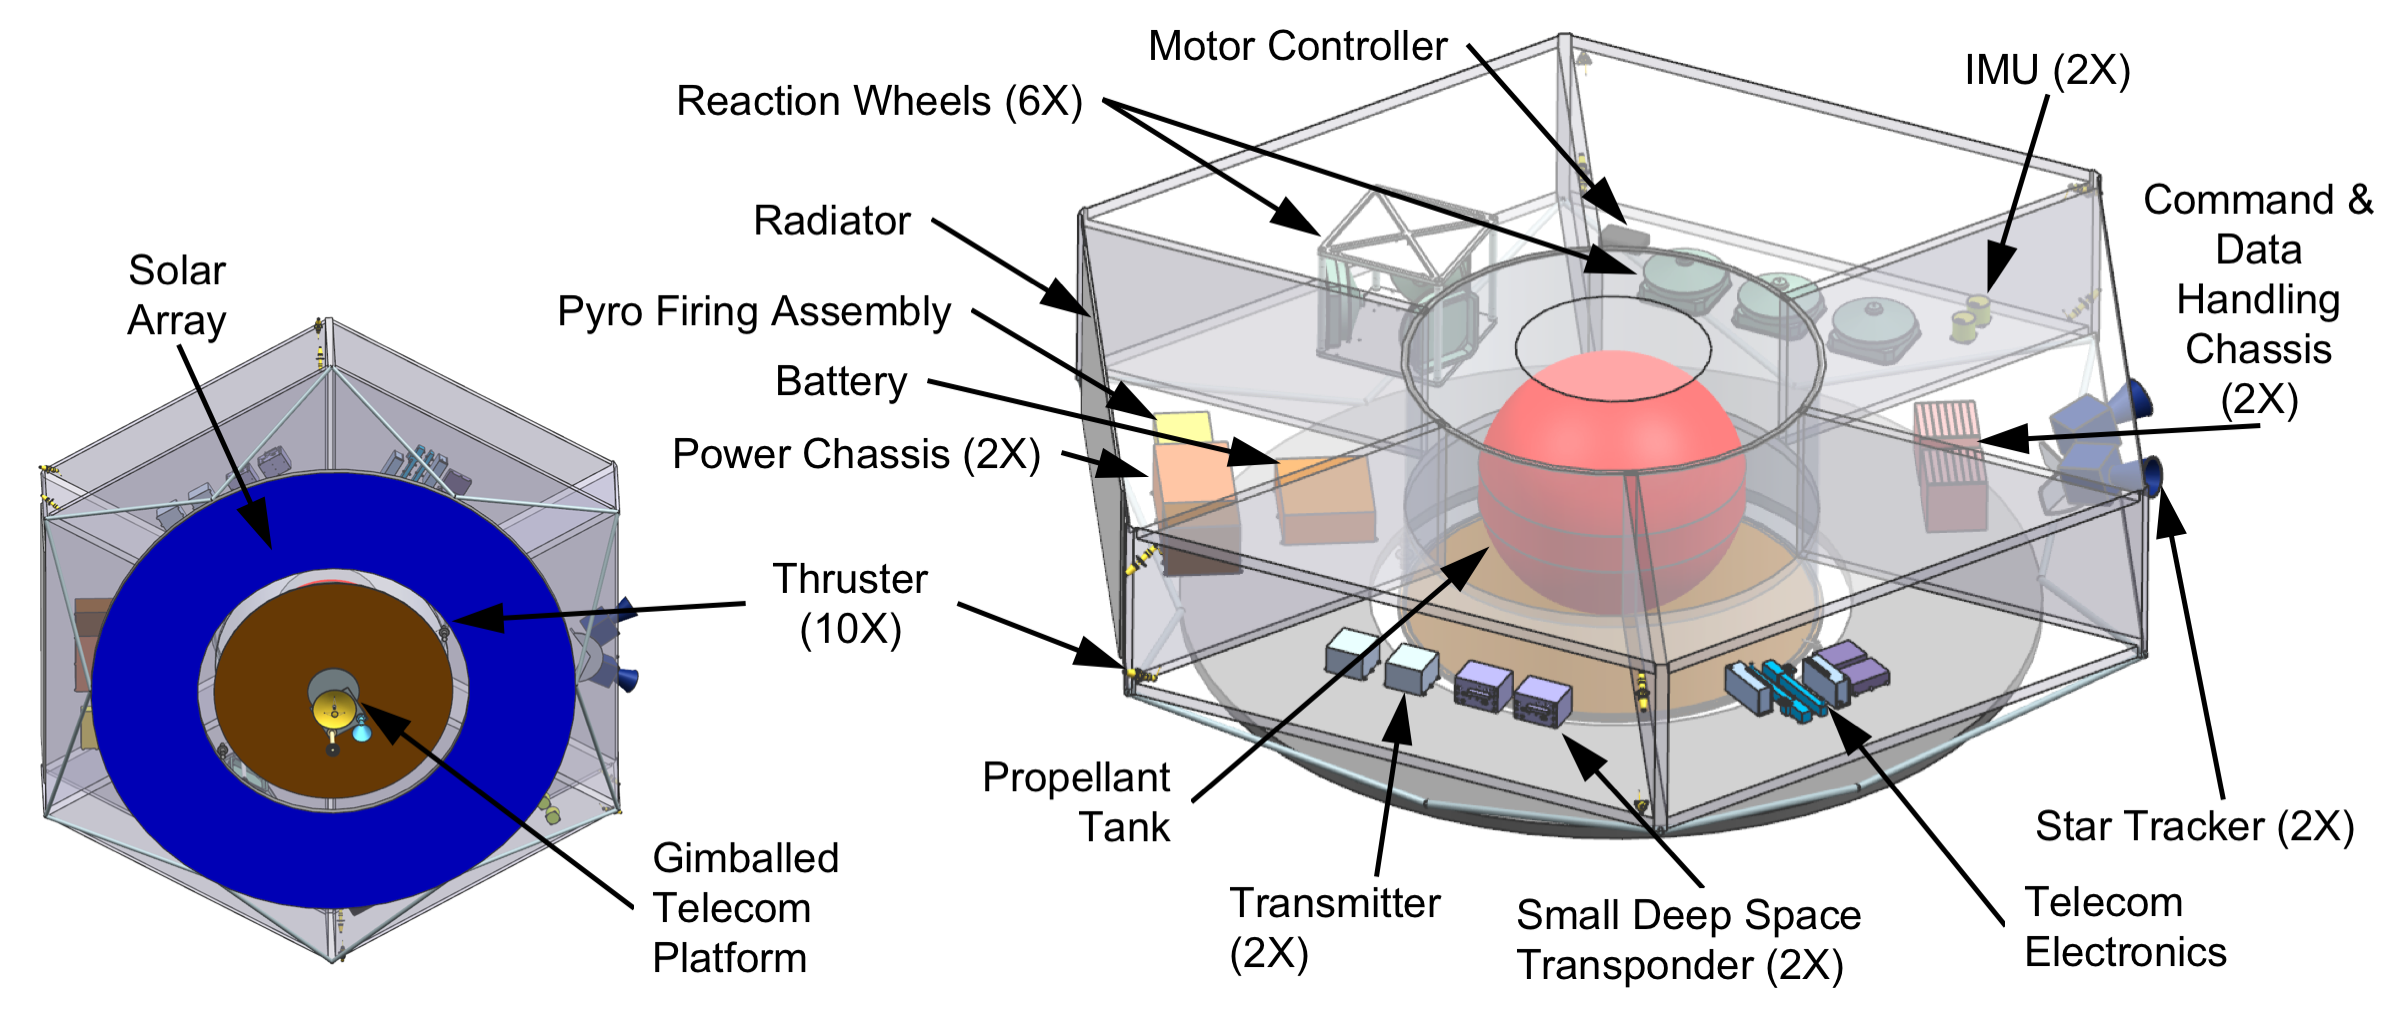
\includegraphics[width=\textwidth]{figures/Spacecraft.png}
\caption{Modular equipment bays provide easy access to all components
  in the spacecraft de-spun module and enable parallel integration of
  spacecraft subsystems.\label{fig:Spacecraft}}
\end{center}
\end{figure}

\subsection{Spacecraft}
\label{sec:spacecraft} %4.3

The PICO spacecraft bus meets all performance requirements with
margin. It is designed for a minimum lifetime of 5\,years in the L2
environment. Mission critical elements are redundant. Flight spares,
engineering models and prototypes appropriate to Class~B are budgeted.

The aft end of the spacecraft (the ``de-spun module'') is comprised of
six equipment bays that house standard components
(Fig.~\ref{fig:Spacecraft}).  The instrument and V-grooves are mounted on
bipods from the spacecraft ``spun module,'' which contains hosted
instrument elements (Fig.~\ref{fig:InstrumentCAD}). A spin motor drives the
spun module at 1\,rpm to support the science survey requirements
(\S\,\ref{sec:survey_design}). Reaction wheels on the despun module
cancel the angular momentum of the spun module and provide three-axis
control (\S\,\ref{sec:attitude_determination}).

The bipods that mechanically support the instrument are thermally
insulating. The passively radiating V-groove assembly thermally
isolates the instrument from solar radiation and from the bus
(\S\,\ref{sec:radiative_cooling}). Like \textit{Planck} \citep{Tauber2010}, the V-grooves are
manufactured using honeycomb material. Additional radiators on the
spun and despun spacecraft modules ($\sim1$\,m$^2$ each) reject heat
dissipated by spacecraft subsystems and hosted instrument elements.

PICO's avionics are dual-string with standard interfaces. Solid state
recorders provide three days of science data storage (ensuring
robustness to missed telecom passes).

PICO employs a fully redundant Ka- and X-band telecommunications
architecture. The Ka-band system uses a 0.3\,m high-gain antenna to
support a science data downlink information rate of 130 Mb/s to a
34\,m BWG DSN ground station with a link margin of 4.8\,dB. The X-band
system provides command and engineering telemetry communication
through all mission phases using medium and low gain
antennas. Amplifiers, switches, and all three antennas are on a
gimballed platform, enabling Ka and X-band downlink concurrent with
science observations.

Solar cells on the aft side of the bus provide positive power (with
contingency) for all mission power modes after launch. The driving
mode is telecom concurrent with science survey. Unused area in the
solar array plane affords significant margin for growth
(Fig.~\ref{fig:Spacecraft}). A Li-ion battery provides power during the
launch phase. The heritage power electronics are dual-string.

The propulsion design is a simple monoprop blow-down hydrazine system
with standard redundancy. Two aft-pointed 22\,N thrusters provide
$\Delta v$ and attitude control for TCMs and orbit maintenance. Eight
4\,N thrusters provide momentum management and backup attitude control
authority.

\subsubsection{Attitude determination and control}
\label{sec:attitude_determination} %4.3.1

PICO uses a zero net angular momentum control architecture with
heritage from the SMAP mission \citep{Brown2016}. PICO's instrument
spin rate (1\,rpm) matches that of the \textit{Planck} mission, but
the precession of the spin axis is much faster (10\,hr vs 6\, months),
and the precession angle much larger ($26\degree$ vs
$7.5\degree$). These differences make the spin-stabilized
\textit{Planck} control architecture impractical because of the amount
of torque required to drive precession.

The PICO 1\,rpm instrument spin rate is achieved and maintained using
a spin motor. The spin motor drive electronics provide the coarse spin
rate knowledge used for controlling the spin rate to meet the
$\pm0.1$\,rpm requirement.

Three reaction wheel assemblies (RWAs) are mounted parallel to the
instrument spin axis and spin opposite to the instrument to achieve
zero net angular momentum and keep the despun module three-axis
stabilized. The spin axis is precessed using three RWAs mounted normal
to the spin axis in a triangle configuration. Each set of three RWAs
is sized such that two could perform the required function, providing
single fault tolerance.

Spin axis pointing and spin rate knowledge are achieved and maintained
using star tracker and inertial measurement unit (IMU) data. The
attitude determination system is single-fault tolerant, with two IMUs
each on the spun and despun modules, and two star trackers each on the
spun and despun modules. Two sun sensors on the despun module are used
for safe-mode contingencies and instrument Sun avoidance. All attitude
control and reconstruction requirements are met, including spin axis
control $< 60$\,arcmin with $< 1$\,arcmin/min stability, and
reconstructed pointing knowledge $< 10$\,arcsec (each axis, $3\sigma$).

\section{Technology maturation}
\label{sec:technology_maturation} %5

PICO's detector and readout technologies have already been substantially matured through complimentary suborbital experiments, and can be developed by the APRA and SAT programs to NASA's Technology Readiness Level (TRL) 5 before Phase~A (October 2023). The 4\,K cryocooler baselined by PICO requires only standard thermal engineering (\S\,\ref{sec:4kcooler}). 

\subsection{Current state of technologies}
\label{sec:current_state} %5.1

PICO builds off of the heritage of the \textit{Planck} HFI
instrument. The white noise of the \textit{Planck} NTD-Ge bolometers
was background-limited in all channels \citep{Planck2014} with a $1/f$
knee at 200--300\,mHz \citep{Planck2018}. Since \textit{Planck},
numerous suborbital experiments have used monolithically fabricated
TES bolometers and multiplexing schemes to field instruments with
thousands of detectors per camera.

\comor{Sentence 2 and onward do not support sentence 1. Need to discuss.}

\comor{Suggest to change the heading below}

\subsubsection{Optical Coupling and Detectors}
\label{sec:detectors_status} %5.1.1

\comor{suggest the rephrase the text below to make it more readable for the uninitiated. Moved sentences around to make argument more logical. And clarified the issue with detectors.}
Suborbital teams have successfully demonstrated a variety of \comor{schemes to couple the incident free-space electromagnetic radiation onto detectors}, including horns with ortho-mode transducers (OMTs), lithographed antenna arrays, and sinuous antennas under lenslets (Fig.~\ref{fig:OpticalCoupling}). In all of these schemes the radiation is coupled through on-wafer transmission lines to bolometric transition-edge sensor detectors. Experiments on the ground and balloons are implementing \comor{these technologies with} many of PICO's observing bands between 30\,GHz and 270\,GHz (Table~\ref{tab:suborbital}). SPT-3G is using the PICO-baselined three-color pixel design to deploy 16,260 detectors covering 90--150--220~GHz \comor{add reference}. \comor{Advanced ActPol} has successfully deployed two-color pixels \comor{add reference}. All of these detector arrays have been packaged into modules and focal plane units in working cameras representative of the PICO integration. The experiments have achieved background-limited performance in both ground and balloon instruments.

To date, suborbital experiments have achieved statistical map depths of 3\,$\mu$K$_{\rm CMB}$\,arcmin on degree-scaled modes over small parts of the sky, approaching what PICO will achieve over the entire sky. Suborbital experiments have also demonstrated systematic control to this level through full-pipeline simulations and null-test analysis (jackknife tests). Moreover, laboratory tests and in-flight data from balloons suggest that these TES bolometers are more naturally robust against cosmic rays than the individual NTD-Ge bolometers used in Planck. Cosmic ray glitches have fast recovery times and low coincidence rates~\citep{SPIDER2018}.
\comor{what did this paragraph want to say? not clear. what does that have to do with the title of the section?} 

\begin{figure}
  \begin{minipage}[b]{0.47\textwidth}
    \begin{center}
    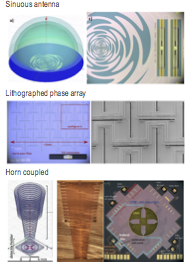
\includegraphics[width=2.5in]{figures/OpticalCoupling.png}
    \caption{Multiple demonstrated optical coupling schemes are available   to PICO. Images from CMB-S4 Technology Book   \citep{Abitbol2017}.\label{fig:OpticalCoupling}}
   \end{center}
  \end{minipage}
  \hspace{0.15in}
  %
  \begin{minipage}[b]{0.47\textwidth}
    \begin{center}
    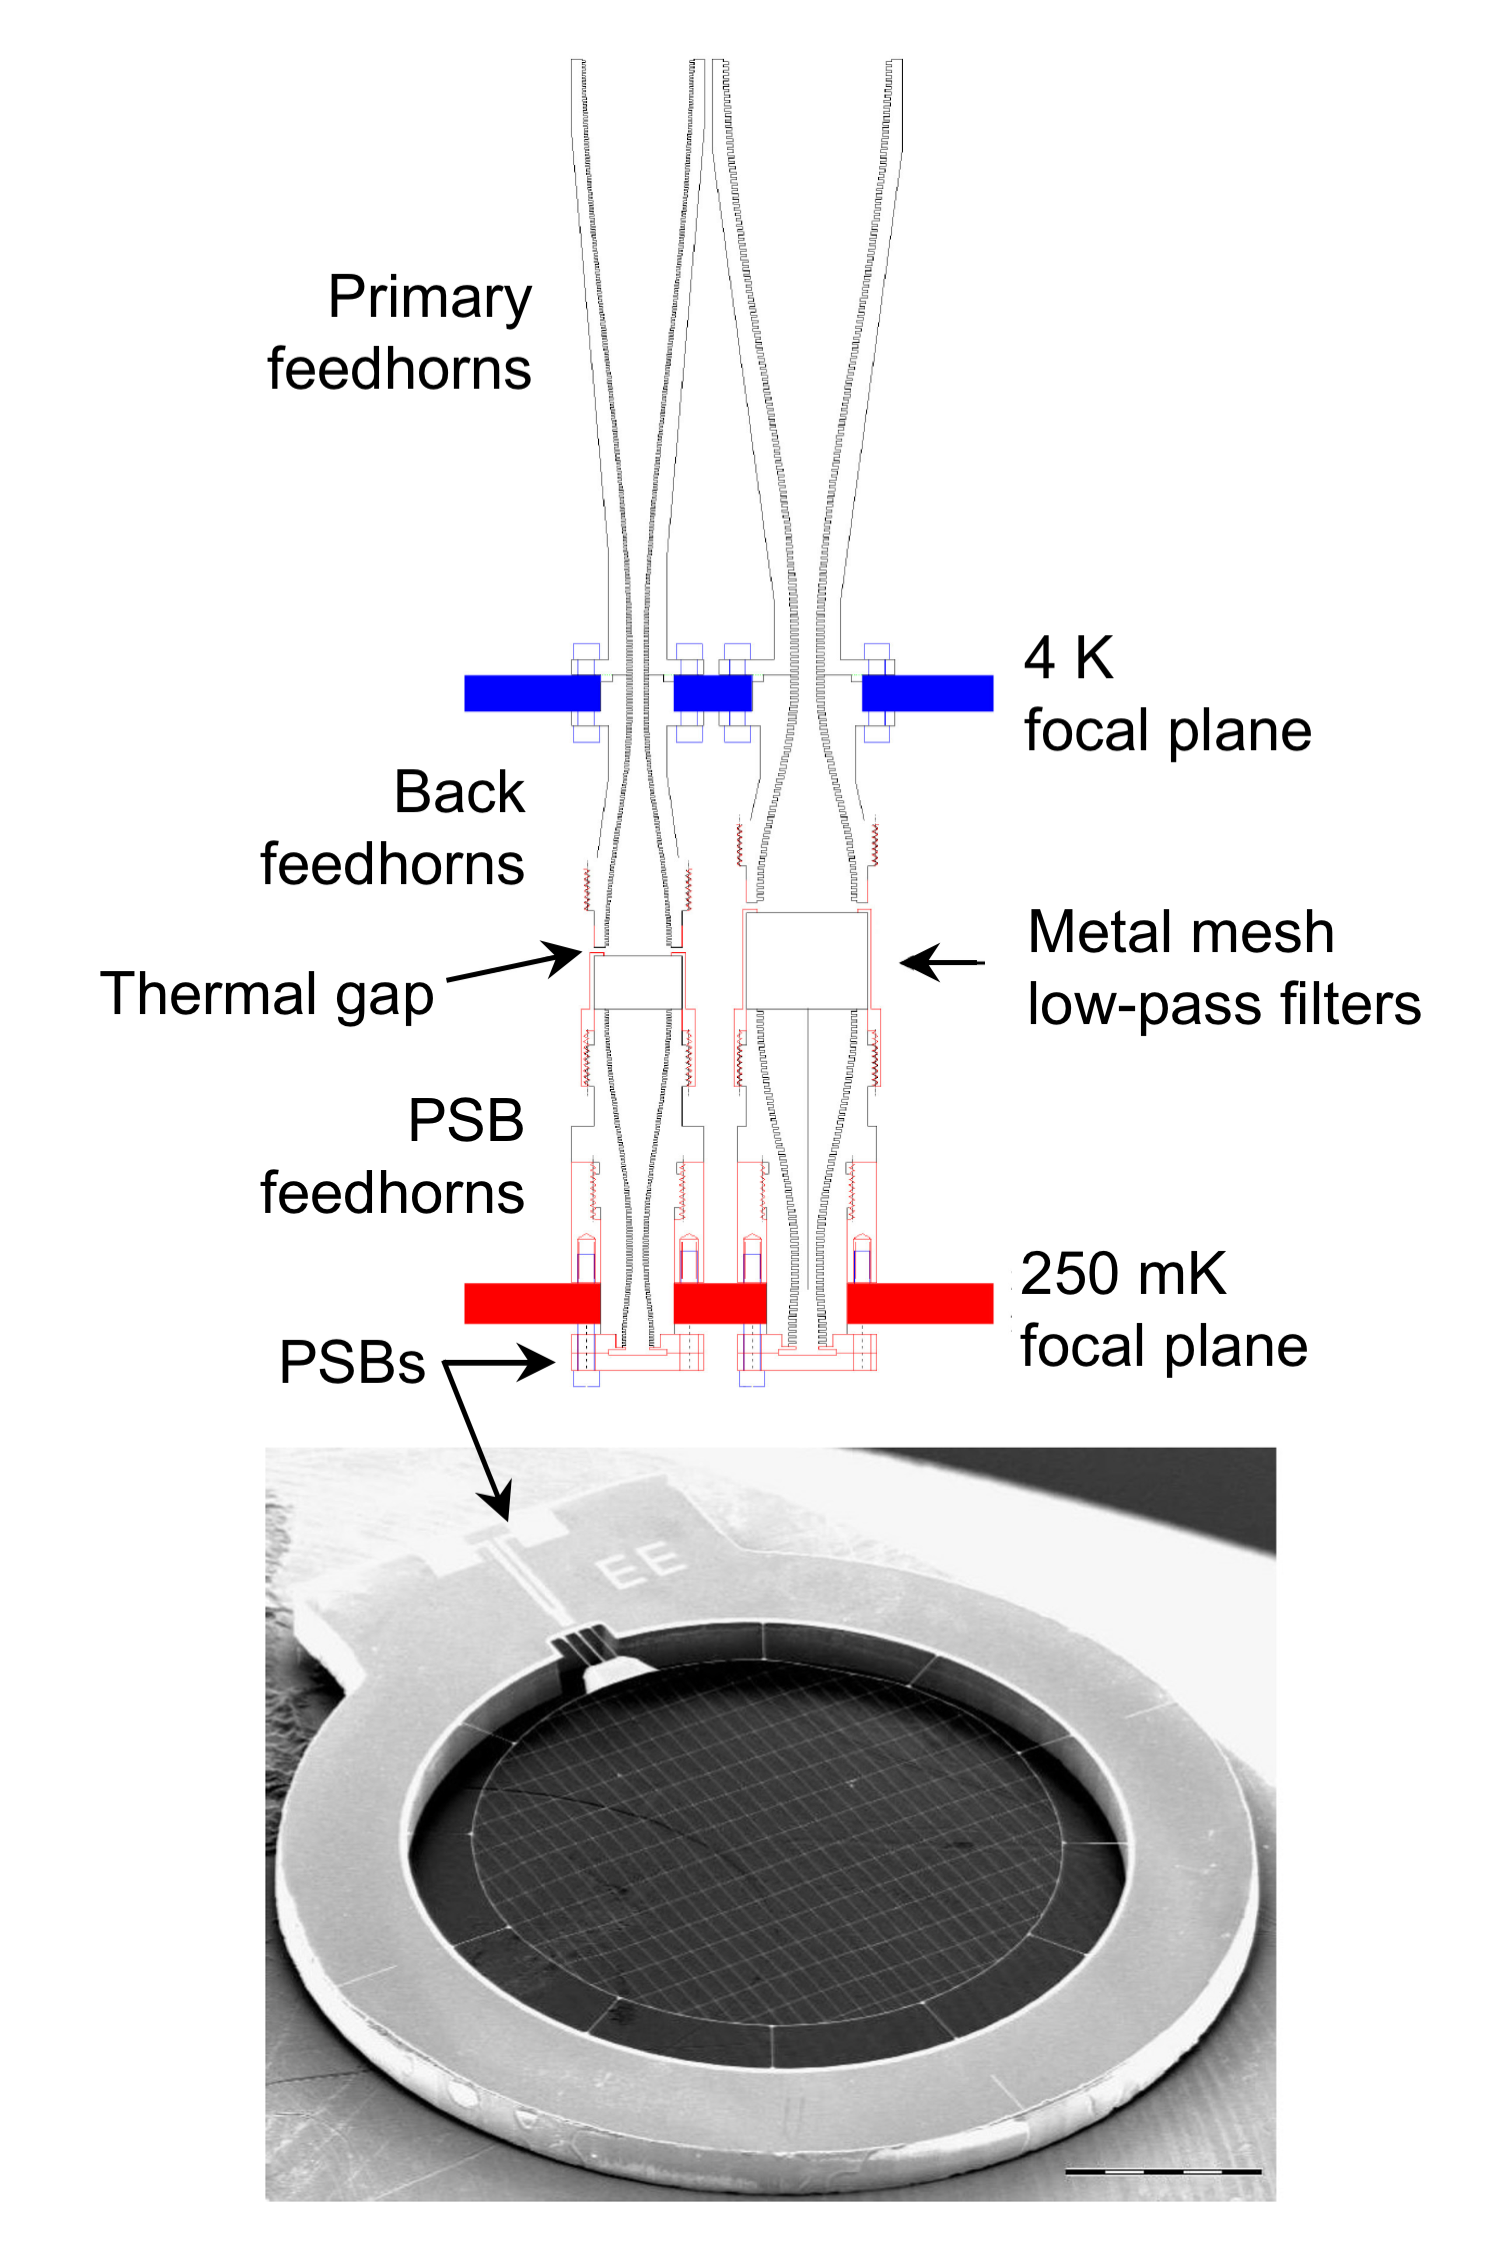
\includegraphics[width=2.5in]{figures/DirectAbsorbing.png}
    \caption{Direct-absorbing dual-polarized detectors and coupling horns used in \textit{Planck} for 143--343\,GHz bands.\label{fig:DirectAbsorbing}}
    \end{center}
  \end{minipage}
\end{figure}

% \begin{figure}
% \begin{center}
% 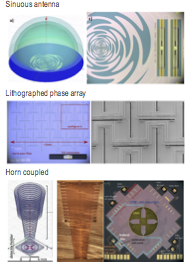
\includegraphics[width=3in]{figures/OpticalCoupling.png}
% \caption{Multiple demonstrated optical coupling schemes are available
%   to PICO. Images from CMB-S4 Technology Book
%   \citep{Abitbol2017}.\label{fig:OpticalCoupling}}
% \end{center}
% \end{figure}

% \begin{figure}
% \begin{center}
% 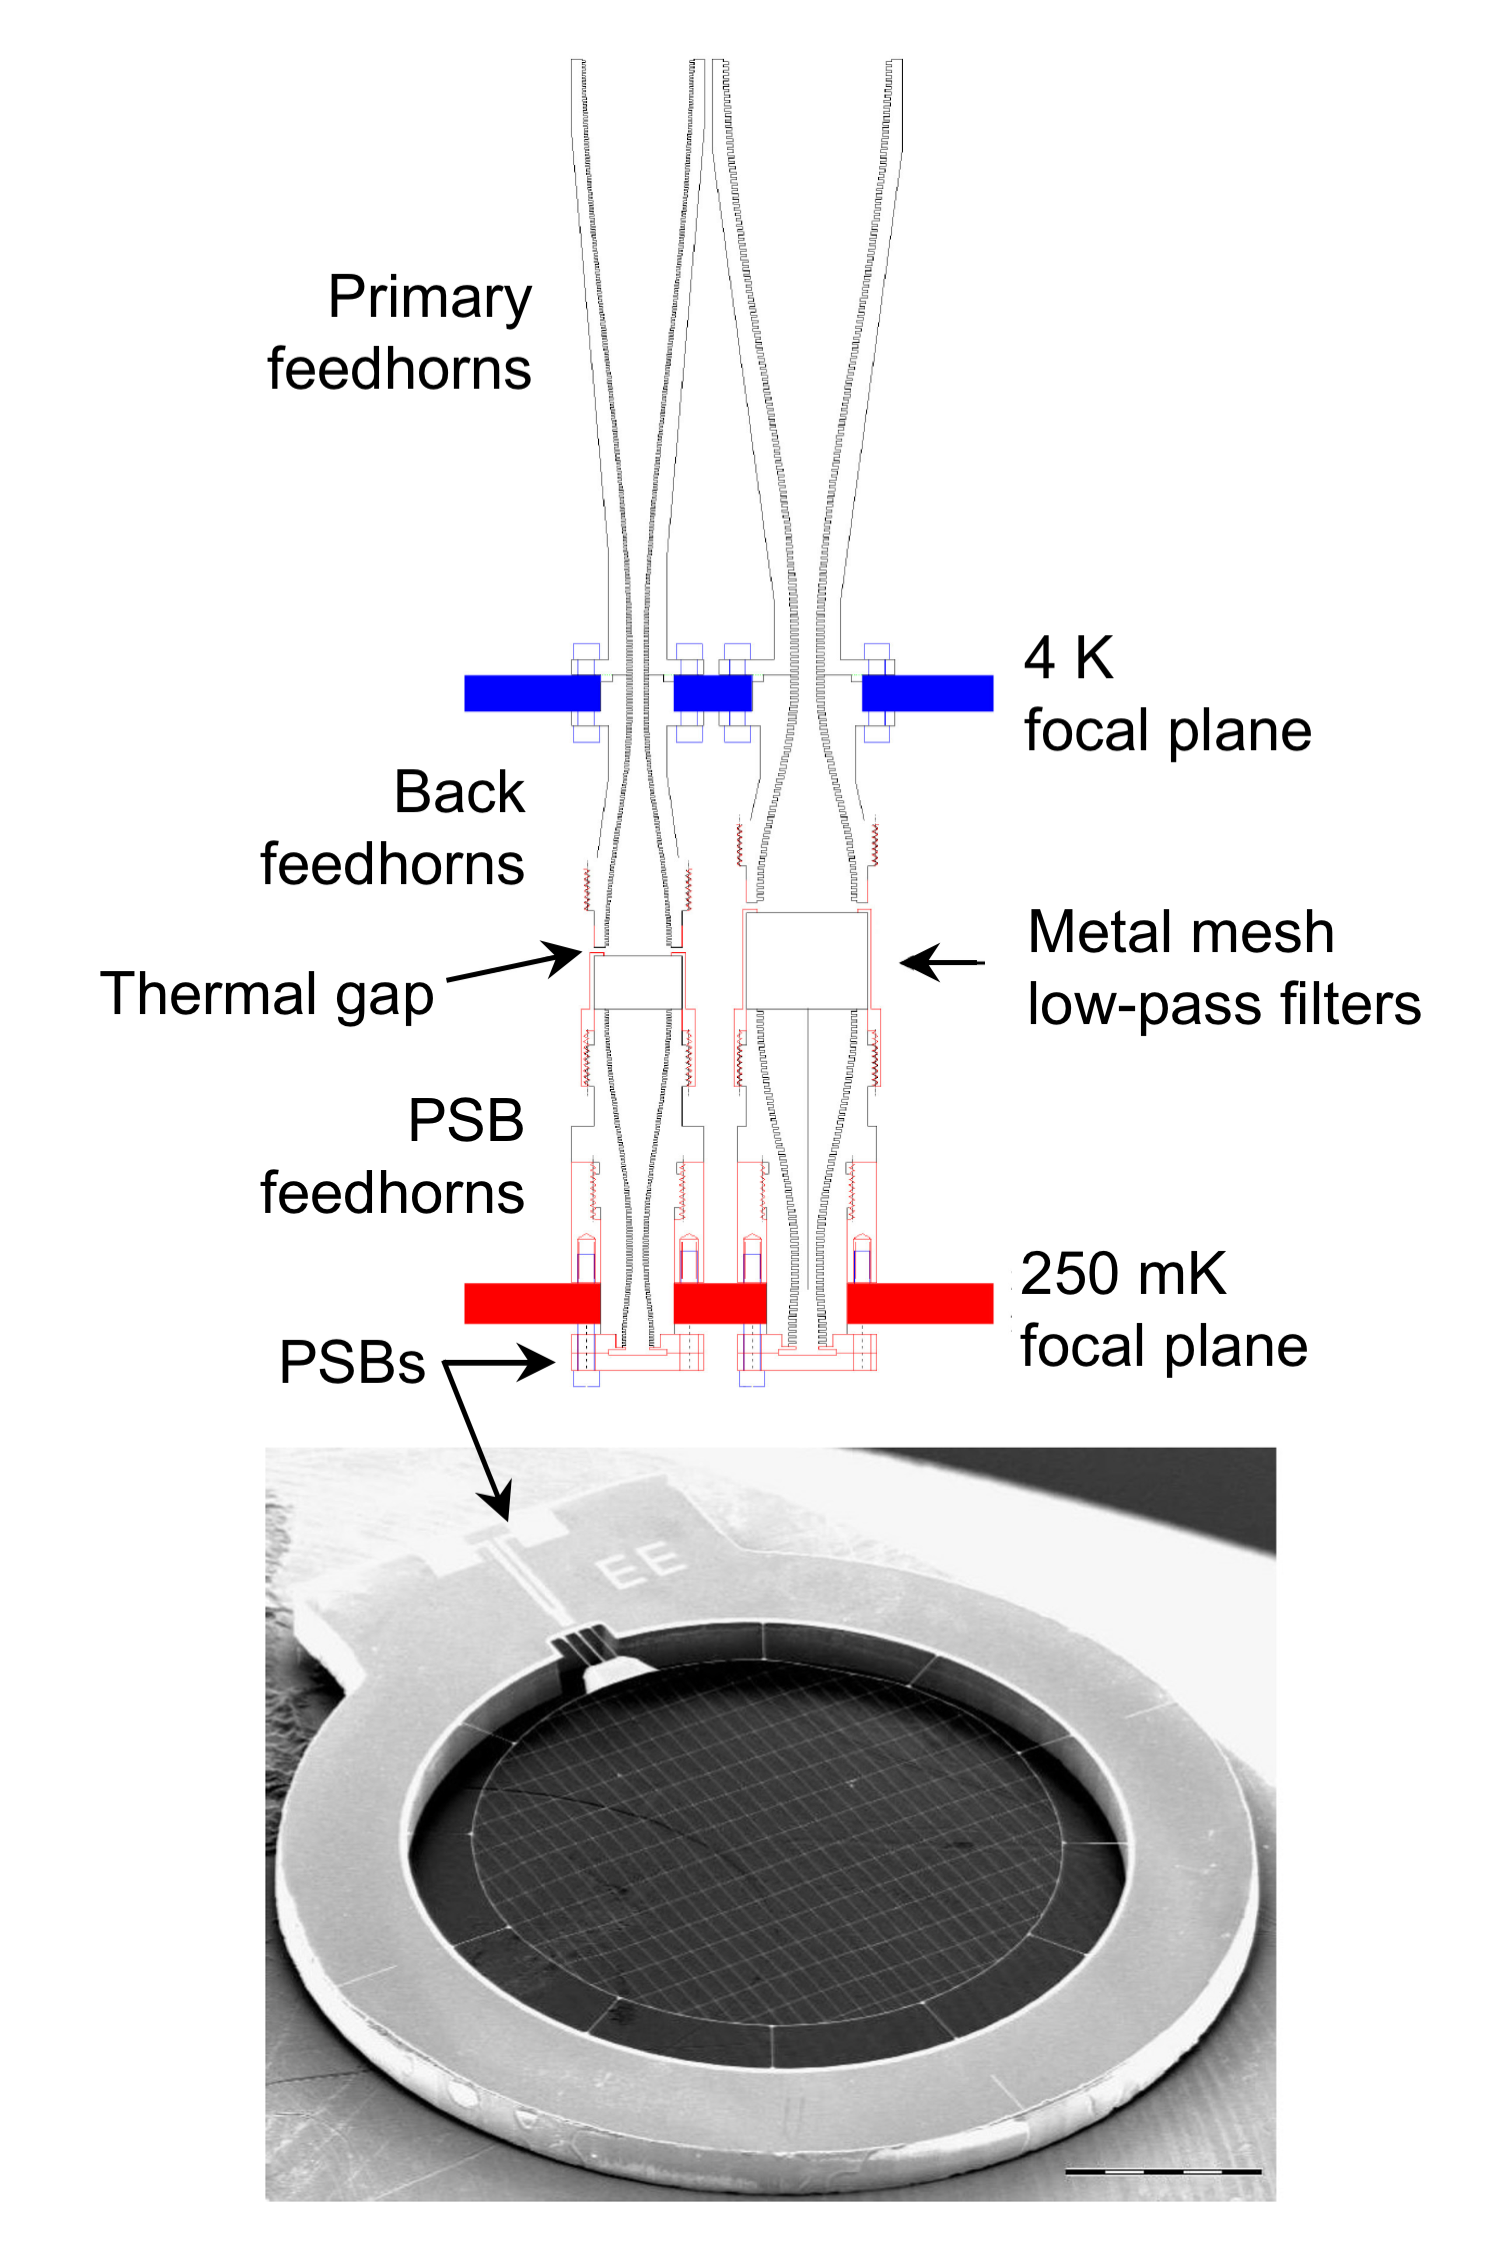
\includegraphics[width=3in]{figures/DirectAbsorbing.png}
% \caption{Direct-absorbing dual-polarized detectors and coupling horns used in \textit{Planck} for 143--343\,GHz bands.\label{fig:DirectAbsorbing}}
% \end{center}
% \end{figure}

PICO's 555--799\,GHz channels (above the Niobium band gap) will use direct absorber bolometers. Ground and balloon experiments have deployed focal planes with hundreds of horn-coupled spiderweb bolometers. SPT-Pol deployed dual-polarized versions of direct absorber horn-coupled bolometers. \textit{Planck} used this style of bolometer, but with NTD-Ge thermistors instead of TESes (Fig.~\ref{fig:DirectAbsorbing}). Filled arrays of detectors such as Backshort Under Ground (BUG) bolometers are also an option for these channels. The status of these efforts is summarized in Table~\ref{tab:suborbital}.
\comor{why are we showing the Planck detectors when we should show Herschel for the higher frequency bands?}

\subsubsection{Readout electronics status}
\label{sec:readout_status} %5.1.2

More than ten experiments have used TDM readout. SCUBA2 on JCMT has 10,000 pixels, nearly as many detectors as planned for PICO \citep{Holland2013}.
\comor{we must also say something about FDM and $\mu$mux. We can't ignore these technologies.} 

\subsection{Development plan}
\label{sec:development_plan}  %5.2

\subsubsection{Detector development}
\label{sec:detector_development} %5.2.1

The baseline PICO instrument requires three-color dual-polarized antenna-coupled bolometers covering bands from 21 to 462\,GHz and single-color dual-polarized direct-absorbing bolometers from 555 to 799~GHz (\S\,\ref{sec:low_freq_det}, \comor{and} Table~\ref{tab:focal_plane}). The developments required to enable the PICO
baseline design are: \\
$\bullet\,\,\,$ extension of antenna-coupled bolometers down to 21\,GHz and up to 462\,GHz; \\
$\bullet\,\,\,$ demonstration of three-color pixels across that spectrum, with characterization of beam properties and associated systematics; \\
$\bullet\,\,\,$ construction of high frequency direct absorbing arrays and laboratory testing; and \\
$\bullet\,\,\,$ beam line and 100\,mK testing to simulate the cosmic ray environment at L2. \\
The extension to lower frequencies requires larger antennas and
therefore control of film properties and lithography over larger
areas. Scaling to higher frequencies forces tighter critical
dimensions and materials tend to exhibit higher losses. These
challenges require tight control of cleanliness and full understanding
of process parameters.
\begin{table}[ht]
\begin{center}
\caption{Multiple active suborbital efforts are advancing technologies relevant to PICO.\label{tab:suborbital}}
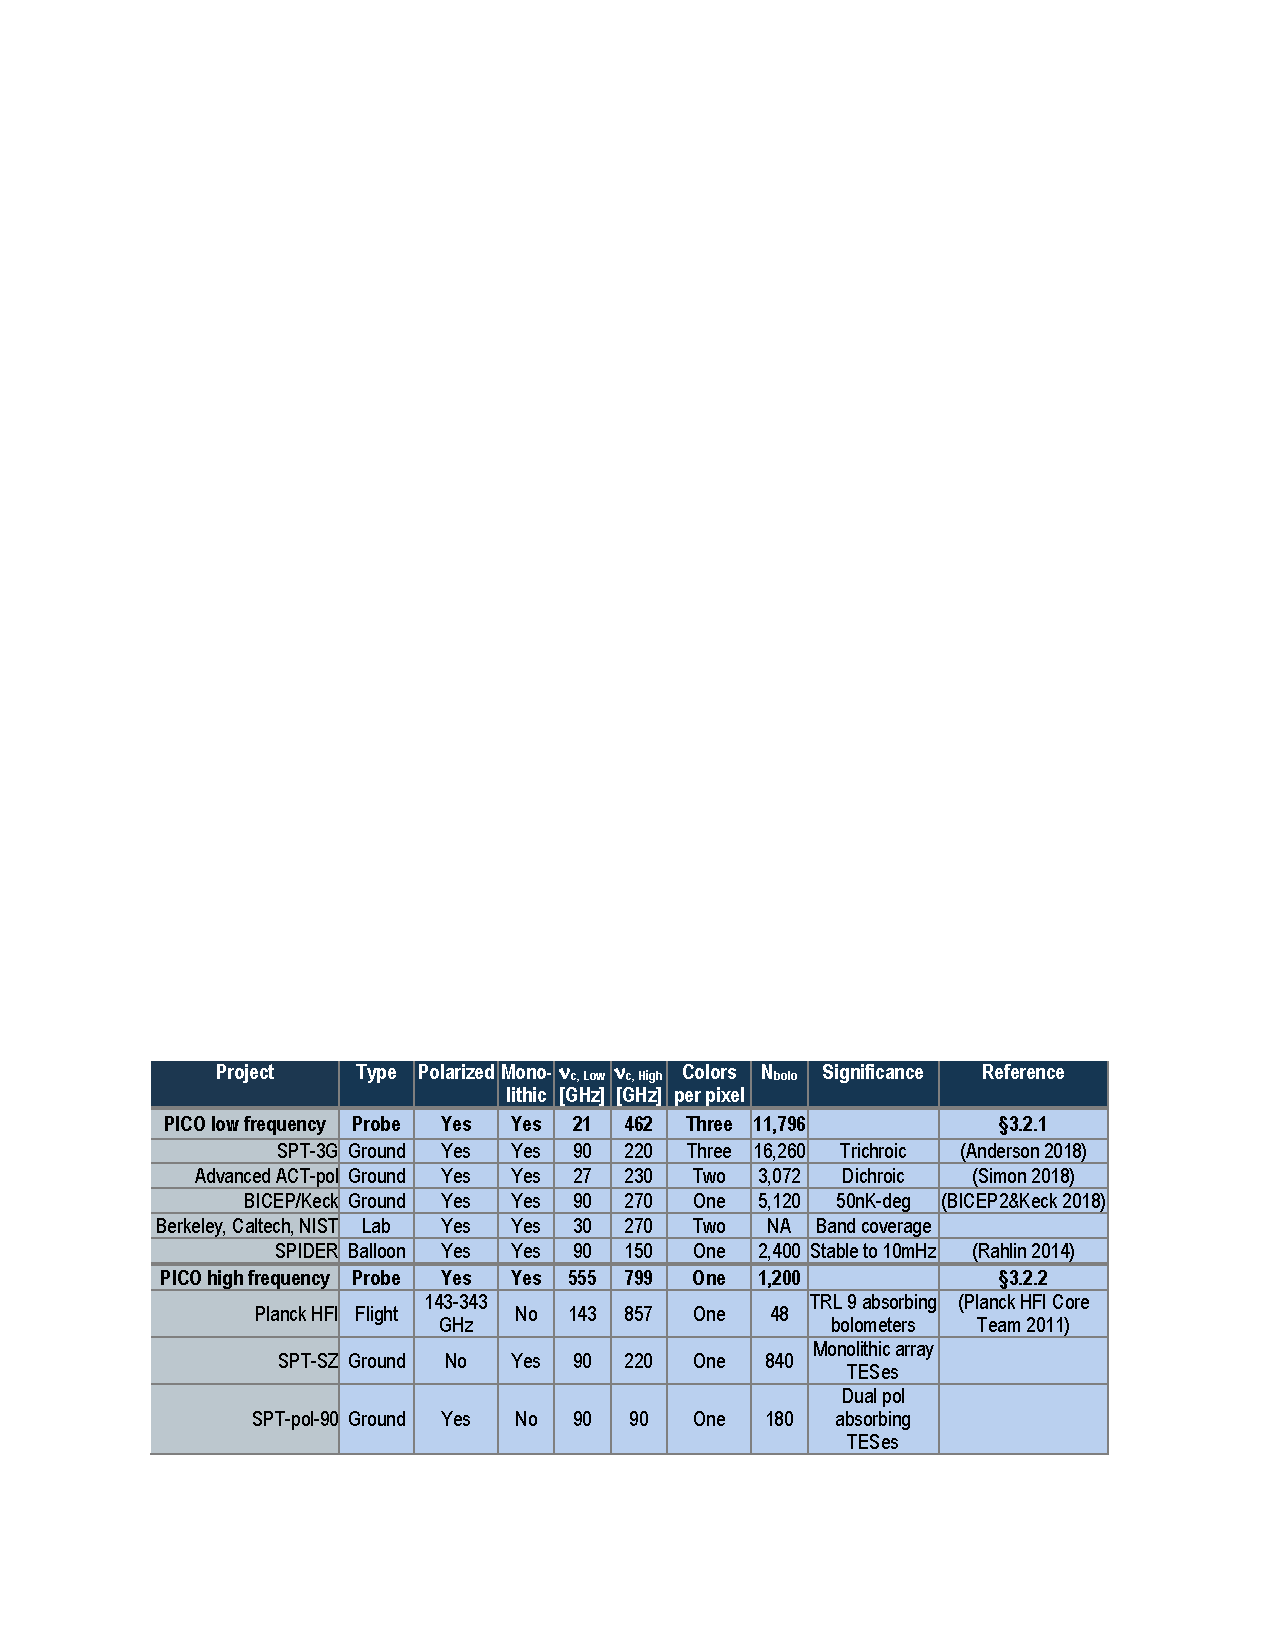
\includegraphics{tables/tab_suborbital.pdf}
\end{center}
\end{table}

The sinuous antenna has the bandwidth to service three-colors per
pixel, whereas horns and antenna arrays have only been used for two,
so some version of the sinuous antenna will likely be needed to
realize three-color pixels. However, the sinuous antenna couples to
states that ``wobble'' log-periodically with frequency. There are
potential solutions to this in the focal plane design, analysis, and
free parameters of the antenna geometry. These will need to be
explored subject to the uniformity and packing density constraints
present at the extreme spectral bands.  Systematics studies for field
demonstrations will be particularly important. The PICO concept is
robust to any challenges in developing three-color pixels;
\S\,\ref{sec:technology_descopes} describes an option to descope to
two-color pixels.

\textit{Planck} demonstrated the architecture of horns coupled to
direct absorbing bolometers. For PICO's high frequency detectors, this
only needs to be generalized to dual polarized arrays. The greatest
remaining challenge is the low risk development of a packaging
design. Such prototyping could culminate in a field demonstration,
best performed in a balloon.

So far, cosmic ray tests and in-flight analysis of TES bolometers are
encouraging \citep{SPIDER2018}. The CMB community can retire residual
risk with 100\,mK testing where the array heat sinking may be weaker,
and beam-line tests to help control for background glitch rates.

A plan to accomplish all required development is described in Table~\ref{tab:technologies}.

\begin{table}
\begin{center}
\caption{PICO technologies can be developed to TRL~5 prior to a 2023 Phase~A start using the APRA and SAT programs.\label{tab:technologies}}
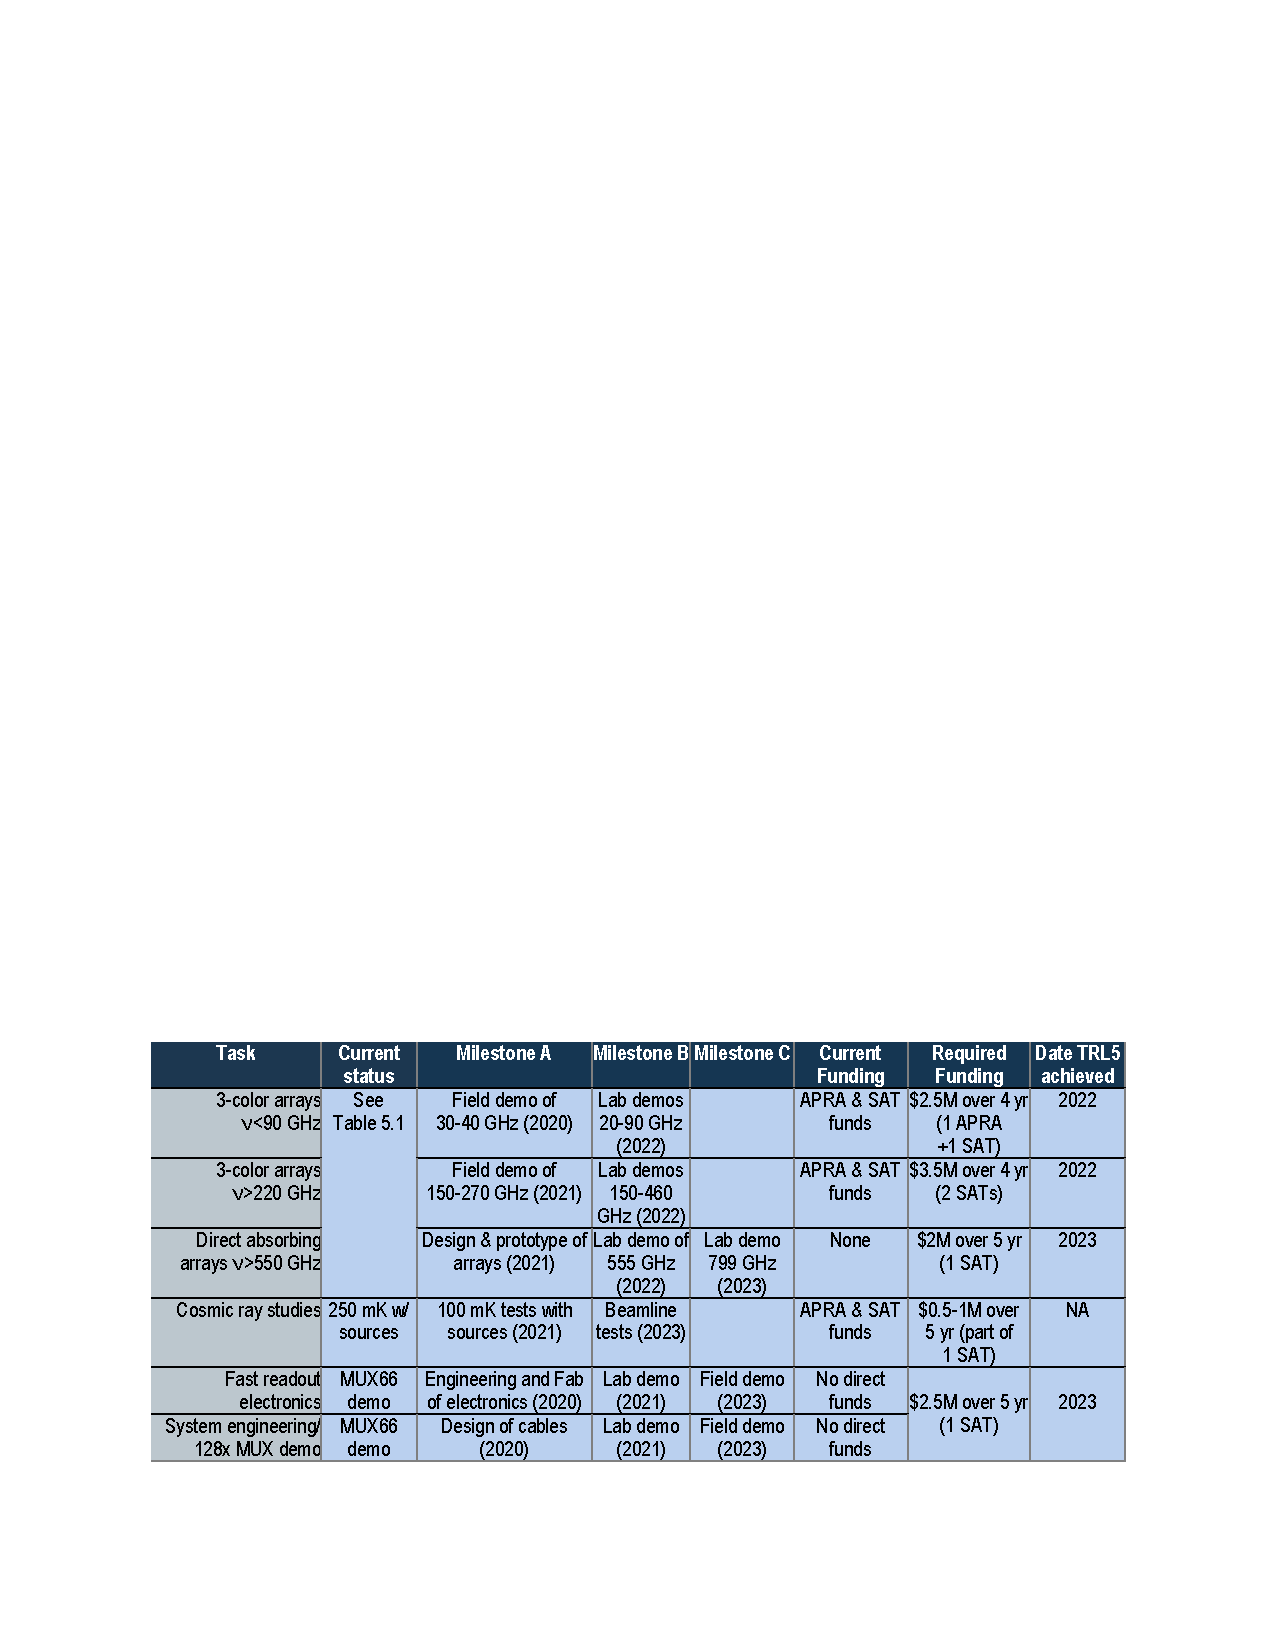
\includegraphics{tables/tab_technologies.pdf}
\end{center}
\end{table}

\subsubsection{Readout electronics development}
\label{sec:readout_development} %5.2.2

PICO's sensitivity requirements dictate the use of $\sim 13,000$ transition edge sensor bolometers, requiring a highly multiplexed system.  The PICO baseline design calls for time division multiplexing with 128 switched rows per readout column (TDM-128$\times$), which exceeds that of Advanced ACTPol's recently demonstrated TDM-66$\times$ \citep{Henderson2016}. The leap to TDM-128$\times$ requires: \\
$\bullet\,\,\,$ development of fast-switched room temperature electronics; \\
$\bullet\,\,\,$ system engineering of room temperature to cryogenic row select cabling to ensure sufficiently fast row switch settling times; and \\
$\bullet\,\,\,$ demonstration of TDM-128$\times$ SQUID aliased noise below PICO detector sensitivity requirements. \\
A plan to accomplish the required development is described in Table~\ref{tab:technologies}.

\subsection{Technology descopes}
\label{sec:technology_descopes} %5.3

A descope from three-color to two-color pixels remains a viable
alternative should the three-color technology not mature as
planned. Descope studies suggest that a PICO-size focal plane using
two-color pixels at the lower frequencies and the baseline one-color
pixels at the higher frequencies would contain 8,840 detectors
(compared to the baseline 12,966) and map in 19 colors (baseline
21). Because horns have a $2.3:1$ bandwidth, each of the two bands in
a pixel has 35\% bandwidth (compared to the baseline 25\%), which
compensates for pixel count, resulting in the same
0.61\,$\mu$K$_{\rm CMB}$\,arcmin aggregate map depth
(Table~\ref{tab:bands}), but with coarser spectral resolution.

\subsection{Enhancing technologies}
\label{sec:enhancing_technologies} %5.4

The following technologies are neither required nor assumed by the
PICO baseline concept. They represent opportunities to extend
scientific capabilities or simplify engineering.

PICO baselines TDM readout because of its relative maturity and
demonstrated sensitivity and stability in relevant science
missions. Lab tests of Frequency Domain Multiplexing (FDM) suggest
comparable performance with higher multiplexing factors and lower
loads on cryogenic stages relative to TDM. Suborbital experiments such
as SPT-3G have used frequency division multiplexing (FDM) to readout
focal planes comparable in size to PICO.

Microwave frequency SQUID multiplexing can increase the multiplexing
density and reduce the number of lines between the 4K and ambient
temperature stages \citep{Dober2017,Irwin2004}. Kinetic Inductance
Detectors (KIDs) and Thermal KIDs (TKIDs) can further reduce the wire
count, obviate the SQUIDs, and dramatically simplify integration by
performing multiplexing on the same substrate as the detectors
themselves \citep{McCarrick2016,Steinbach2018}. The cost to develop
these technologies is \$3--4M/year, with a high chance of reaching
TRL-5 before Phase~A.

\section{Project management, heritage, risk, and cost}
\label{sec:project_management} %6

\subsection{PICO Study Participants}
\label{sec:study_participants} %6.1

The PICO study was open to the entire mm/sub-mm science community and
included more than 150 scientists. Seven working groups were led by
members of PICO's Executive Committee, which met weekly under the
leadership of PI Shaul Hanany. More than 60 people participated
in-person in two community workshops (November 2017 and May 2018).

The PICO engineering concept definition package was generated by
Team~X (the JPL concurrent design lab). The Team X study was supported
by inputs from a JPL engineering team and Lockheed Martin.

The full list of study report contributors and endorsers follows the cover page.

\subsection{Project management plan}
\label{sec:management_plan} %6.2

PICO benefits from the experience of predecessor missions such as
\textit{Planck} and \textit{WMAP}, as well as many years of investment
in technology development and a multitude of suborbital
experiments. In addition to demonstrated science and engineering
capabilities, this heritage has developed a community of people with
the expertise required to field a successful mission.

This study assumes mission management by JPL with a Principal
Investigator leading a single science team. A Project Manager provides
project oversight for schedule, budget, and deliverables. A Project
Systems Engineer leads systems engineering activities and serves as
the Engineering Technical Authority. A Mission Assurance Manager
serves as the Independent Technical Authority. The PICO mission
development schedule is shown in Fig.~\ref{fig:Schedule}.

\begin{figure}[hb]
\begin{center}
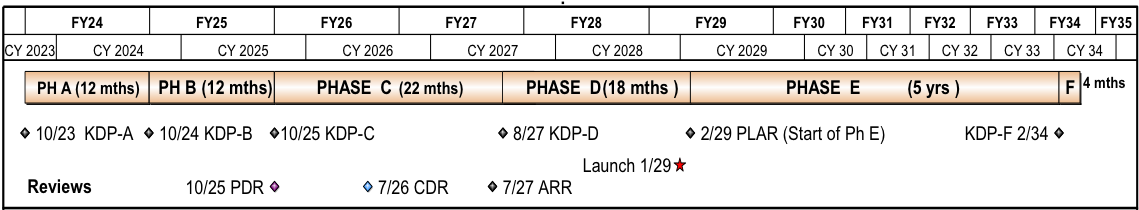
\includegraphics[width=\textwidth]{figures/Schedule.png}
\caption{The PICO baseline schedule is based on historical actuals
  from similarly-sized missions such as Juno and
  SMAP.\label{fig:Schedule}}
\end{center}
\end{figure}

Probes are medium-class missions, similar in cost scope to NASA's
New Frontiers missions, which are Category~1 and Risk Classification A
or B, with Phase A--D costs capped at $\sim$ \$850M (not including the
launch vehicle). JPL is well-prepared to manage Probe missions, having
managed the Juno New Frontiers mission (launched 2011) and also the
development of the medium-class \textit{Spitzer} Space Telescope (launched
2003). JPL delivered the bolometric detectors for the \textit{Planck}
HFI instrument (launched 2009). Presently, JPL is managing NEOCam, a
Discovery class infrared space telescope.

The PICO spacecraft provider will be selected during mission
formulation. Multiple organizations are capable of providing a
spacecraft bus to meet PICO's requirements. Lockheed Martin
contributed to the PICO concept study, leveraging their experience
with New Frontiers missions Juno and OSIRIS-REx.
 
\subsection{Heritage}
\label{sec:heritage} %6.3

The successful \textit{Planck} mission provides science heritage for
PICO. Technical heritage traces to multiple missions.

Because PICO observes in the mm/sub-mm regime, the surface accuracy
requirement for the reflectors is relatively easy to meet. PICO's
reflectors are similar to \textit{Planck}'s, but somewhat larger
($270\,{\rm cm} \times 205\,{\rm cm}$ primary vs.\
$189\,{\rm cm} \times 155\,{\rm cm}$)
\citep{Gloesener2006}. \textit{Herschel} observed at wavelengths more
demanding than PICO's and was larger ($350\,{\rm cm}$ diameter
primary) \citep{Toulemont2004}.

The heritage of the PICO detectors and readout electronics
(\S\,\ref{sec:focal_plane}, \S\,\ref{sec:detector_readout}) is
described in \S\,\ref{sec:current_state}.


PICO's detectors are cooled by a cADR (\ref{sec:cadr}) with
requirements that are within the capabilities of current cADRs
developed by Goddard Space Flight Center. These systems have been
applied to several JAXA missions, including Hitomi \citep{Shirron2016}.

PICO's 4\,K cryocooler (\S\,\ref{sec:4kcooler}) is a direct extension
of the JWST MIRI design \citep{Durand2008,Rabb2013}. PICO benefits
from a simpler and more reliable implementation of the J-T system than
was required for MIRI, in that no deployment of cooling lines is
required, and all flow valving is performed on the warm
spacecraft. Cooling multiple independent points with a J-T loop has
been demonstrated on \textit{Planck} with the JPL-supplied 18\,K
cooler \citep{Planck2011}.

Structures similar to PICO's V-groove assembly
(\S\,\ref{sec:radiative_cooling}) are a standard approach for passive
cooling first described more than thirty years ago
\citep{Bard1987}. The JWST mission will deploy a
$22\,{\rm m} \times 10\,{\rm m}$ V-groove sun shield. PICO's
relatively modest 4.5\,m diameter V-groove assembly fits inside the
launch vehicle fairing. Because it does not require deployment, PICO
has baselined a simple honeycomb material construction like that
successfully flown by the \textit{Planck} mission
\citep{ESA2009,Planck2011}.

Most requirements on the PICO spacecraft are well within typical
ranges and can be met with standard high heritage systems
(\S\,\ref{sec:spacecraft}). PICO's spin architecture and data volume
requirements are less typical, and discussed below.

The PICO zero-momentum control architecture
(\S\,\ref{sec:attitude_determination}) has heritage from the SMAP
mission. PICO has a slower spin rate and less cancelled angular
momentum than SMAP. SMAP requires 359\,Nms to cancel the momentum of a
6\,m instrument antenna spun at 14.6\,rpm \citep{Brown2016}. The PICO launch
mass (including contingency) is similar to the \textit{Planck} launch mass. If
we assume \textit{Planck} moments of inertia \citep{ESA2016}, the PICO spun elements
would have an angular momentum of 210\,Nms at 1\,rpm. This is
conservative because, unlike \textit{Planck}, the entire PICO
observatory does not spin.

Though PICO's data volume is notable by current standards, it is
already enveloped by missions in development. PICO produces
6.1\,Tb/day of raw data which is compressed to 1.5\.Tb/day
(\S\,\ref{sec:detector_readout}). PICO downlinks data daily, but
baselines storage of 3\,days of (compressed) data to mitigate missed
telecom passes. This requires 4.5\,Tb of onboard storage, in family
with the 3.14\,Tb solid state recorder currently in use by Landsat~8
and much smaller than the 12\,Tbit flash memory planned for NISAR
\citep{Jasper2017}. The PICO baseline 150\,Mb/s Ka-band data downlink
is an existing DSN catalog service (DSN 2015). The TESS mission
presently downlinks data to the DSN using Ka-band at 100\,Mb/s. The
baseline PICO mission generates $\sim2,200$\,Tb of raw (uncompressed)
data per year, less than the $\sim6,800$\,Tb/year currently returned
by Landsat~8 and $\sim 9,300$\,Tb/yr planned by NISAR
\citep{Jasper2017}.

\subsection{Risk assessment}
\label{sec:risk_assessment} %6.4

\subsubsection{Pre-mission risks}
\label{sec:premission_risks} %6.4.1

Technology development (\S\,\ref{sec:technology_maturation}) is
performed prior to the beginning of mission development, and is
outside of the mission cost (per NASA direction), so associated risks
do not represent threats to the cost of mission development. Rather,
they represent risks to the availability of the described baseline
mission. A technology-related mission descope is described in
\S\,\ref{sec:technology_descopes}.

\subsubsection{Development risks}
\label{sec:development_risks} %6.4.2

PICO's healthy contingencies, margins, and reserves provide
flexibility to address risks realized during mission development. PICO
carries $>40\,\%$ instrument sensitivity margin (Table~\ref{tab:bands}),
$>100\,\%$ heat lift margin (Table~\ref{tab:cooler}), $43\,\%$ system
power contingency, $31\,\%$ payload mass contingency, and $27\,\%$
spacecraft mass contingency. The Falcon~9 launch capability (for ocean
recovery) exceeds PICO's total launch mass (including contingency) by
a $\sim 50\,\%$ margin. The PICO budget includes $30\,\%$ cost
reserves for Phases A--D (\S\,\ref{sec:mission_cost}).

During mission development the Project Systems Engineer continually
assesses risks, tracks progress toward retiring them, and updates
mitigations. Mitigations for a few top risks identified during this
study are described below.

Thermal risk can be mitigated through extensive thermal modeling and
review in Phase A, and design for early test verification. Risks
associated with the instrument spin architecture can be mitigated by
engaging JPL engineers who were involved in the SMAP mission. Detector
delivery schedule risk can be mitigated by beginning fabrication early
in the project life cycle and fabricating a generous number of
detector wafers to ensure adequate yield. Risks associated with the
integration and test of a cryogenic instrument can be mitigated
through advanced planning and allocation of appropriate schedule and
schedule margin.

\subsubsection{Operations risks}
\label{sec:operations_risks} %6.4.3

The PICO design meets the requirements associated with the NASA
Class~B risk classification. For Class~B missions, essential
spacecraft and instrument functions are typically fully
redundant. This increases mission cost, but significantly reduces the
risk of mission failure during operations.

The PICO mission utilizes a single instrument with a single observing
mode mapping the sky using a repetitive survey pattern. The mission
does not require any time-critical activities. The observatory fits in
to the launch vehicle fairing in its operational configuration, so no
hardware deployments are required. The telescope does not require a
cover (nor the associated mission-critical cover release).

The spacecraft incorporates a fault protection system for anomaly
detection and resolution. The Sun-pointed, command receptive,
thermally stable safe-mode attitude allows ground intervention for
fault resolution without time constraints. PICO's high degree of
hardware redundancy and onboard fault protection ensure spacecraft
safety in the event of unforeseen failures and faults.

Science data analysis, including foreground separation
(\S\,\ref{sec:2.5}) and systematics control (\S\,\ref{sec:2.6}) are
discussed in the science section (\S\,\ref{sec:2}).

\subsection{Mission cost}
\label{sec:mission_cost} %6.5
 
\textit{The cost section is excluded from this draft release.}

